% Template per tesi di laurea
%
% Creato da Giulio Spinozzi
% giuliospinozzi@gmail.com
% http://giuliospinozzi.altervista.org
%
\documentclass [11pt,a4paper,oneside,openany]{book} %Classe del documento, formato carta, singola facciata, apertura capitoli pag destra/sinista (ininfluente se impostato oneside). Formato libro
%%\usepackage[italian]{babel} %Lingua Documento (da impostare per la sillabazione)
\usepackage{graphicx} %Pacchetto necessario per la gestione delle immagini
\usepackage {fancyhdr} %Pacchetto per la gestione accurata della pagina
\usepackage {setspace} %Pacchetto necessario per i comandi successivi onehalfspacing, singlespacing....
\usepackage{longtable} %Pacchetto per la gestione delle tabelle grandi
\usepackage[colorlinks=true]{hyperref} %Segnalibri nel pdf finale, sotto relativi parametri
\usepackage[italian]{babel}
\usepackage{listings}
\hypersetup{
	bookmarksnumbered=true,
	linkcolor=black,
	citecolor=black,
	urlcolor=black,
}

\usepackage{geometry} % Dimensione pagina
\geometry{a4paper} % Formato carta
\addtolength{\textheight}{75pt} %Margini
\oddsidemargin 30pt


\begin{document} %Inizio Documento

%%FRONTESPIZIO%%=========================================
\begin{titlepage}
 \begin{center}
     
\includegraphics[width=0.65
     \textwidth, keepaspectratio]{fig/logounipg2021}\\ %Logo dell'Universit�, cambiare il percorso, se necessario	\includegraphics[width=0.87
     \vspace{1em}
%     {\Large \textsc{Universit\`a degli Studi di Perugia}}\\
     \vspace{2em}
     {\normalsize Tesi di Laurea in}\\
     \vspace{1em}
     {\Large \textsc{INGEGNERIA INFORMATICA ED ELETTRONICA}}\\
     \vspace{8em}
     {\LARGE \textbf{Sviluppo di un blog decentralizzato tramite tecnologia Solid}}\\
 \end{center}
 
 \vskip 2.5cm
  \begin{center}
    \begin{tabular}{c c c c c c c c}
      Relatore & & & & & & & Candidato \\[0.2cm]
      \Large{\textit{Luca Grilli}} & & & & & & & \Large{\textit{Carlo Tosoni}}\\[0.4cm]
    \end{tabular}
  \end{center}

\vskip 2.5cm
\begin{center}
{\normalsize Anno Accademico 2020/2021}
\end{center}
\end{titlepage}

%%DEDICA%%=============================================
\pagestyle{empty}
\vspace{5em}
\begin{flushright}
{\Large \textit{}}
\end{flushright}

\newpage

%%INTESTAZIONI PAGINA%%====================================
\pagestyle{fancy}
\renewcommand{\chaptermark} [1]{\chaptername\ \thechapter.\ #1}{} 
\renewcommand{\chaptermark}[1]{\markboth{\thechapter.\ #1}{}} 
\renewcommand{\sectionmark}[1]{\markright{\thesection\ #1}}
\fancyhf{}
\fancyhead[LE,RO]{\bfseries\thepage} 
\fancyhead[LO,RE]{\bfseries\leftmark} 
\fancypagestyle{plain}{%
\fancyhead{} % leva l'intestazione
\renewcommand{\headrulewidth}{0pt} % e la linea
}


%%INDICE%%==============================================
\tableofcontents

%%CAPITOLI===============================================
\onehalfspacing

\chapter{Introduzione}

\medskip

Il 6 agosto 1991 venne inventata una delle tecnologie più importanti del secolo, destinata a rivoluzionare la società: questa invenzione è il {\tt World Wide Web}. In quel giorno, l'informatico inglese Sir Tim Berners-Lee, fondatore del web, pubblicò presso il CERN di Ginevra il primo sito internet della storia che descriveva il progetto {\tt WWW}. 17 giorni dopo il sito venne per la prima volta visitato da un utente esterno al centro di ricerca; da quel giorno il web si diffuse sempre di più, espandendosi ad una velocità impressionante. Oggi, nell'anno 2021, dei circa 7.83 miliardi di persone esistenti al mondo, ben 4.66 miliardi hanno accesso ad internet, per un numero complessivo di utenti che è pari a il 59.5\% della popolazione mondiale totale \cite{wearesocial}. Berners-Lee aveva originariamente immaginato il web come: "una piattaforma aperta che avrebbe permesso a tutti, ovunque, di condividere informazioni, di accedere ad opportunità e di collaborare attraverso differenti aree geografiche e confini culturali" \cite{worldwideweb}. Questa visione di Berners-Lee è tuttavia venuta a mancare con il passare degli anni, in quanto il web è diventato un luogo sempre più posto sotto il diretto controllo delle grandi multinazionali, le quali, attraverso il possesso dei dati degli utenti, monopolizzano la rete, impedendo agli utenti stessi di essere i reali proprietari del web. A seguito dello scoppio di alcuni scandali, come ad esempio quello relativo a Facebook-Cambridge Analytica \cite{facebook}, i quali hanno messo in evidenza le violazioni perpetuate da alcuni dei grandi colossi del web ai danni degli utenti di internet e della loro privacy, Berners-Lee ha deciso, in collaborazione col MIT di Boston, di fondare un nuovo progetto finalizzato a ridecentralizzare il web, esattamente come lo aveva immaginato il su fondatore nella sua visione originale. Tale progetto, che prende il nome di {\tt Solid} (Social Linked Data), mira a dividere il piano delle applicazioni da quello dei dati, permettendo agli utenti di controllare in maniera diretta i propri dati personali, senza lasciarli sotto il controllo delle grandi multinazionali. {\tt Solid} è una specifica che permette agli utenti di salvare i propri dati in sicurezza all'interno di archivi di dati decentralizzati chiamati {\tt Pod}. I {\tt Pod} sono come dei server web personali e sicuri per la memorizzazione dei dati dell'utente. Una volta salvati i dati all'interno del {\tt Pod} di un utente, costui è in grado di controllare quali applicazioni e quali altri utenti possono avere accesso a tali dati. {\tt Solid} mira quindi a "cambiare il modo in cui funzionano le attuali applicazioni Web, per ottenere un reale possesso dei dati ed una maggiore privacy da parte degli utenti" \cite{mitsolid}. Allo stato attuale, questa tecnologia risuta, tuttavia, essere ancora in fase di sviluppo.

\bigskip

Il presente progetto di tesi è finalizzato alla creazione di applicazioni decentralizzate utilizzando la tecnologia {\tt Solid}, con il fine di evidenziare i vantaggi dovuti al loro utilizzo e di mostrare le differenze tra una normale applicazione ed una decentralizzata. Poiché le applicazioni decentralizzate non salvano localmente alcun dato relativo all'utente, quest'ultimo è portato a scegliere quali applicazioni utilizzare soltanto in base alla qualità del servizio che queste offrono e non per il possesso esclusivo dei suoi dati. A tal proposito ogni dato salvato all'interno del {\tt Pod} può essere riutilizzato dagli utenti in base alle loro necessità, permettendo eventualmente ad altre applicazioni di accedervi o di revocarne i permessi, in lettura o in scrittura, precedemente concessi ad applicazioni o utenti.

\bigskip


Nello specifico, il presente elaborato di tesi è finalizzato allo sviluppo di due differenti applicazioni che formano il sistema denominato {\tt SADeB} (Solid Authenticity Decentralized Blog). Il sistema {\tt SADeB} ha lo scopo di mettere in evidenza il funzionamento di un'applicazione {\tt Solid}, mostrando le modalità con cui un utente può permettere ad un'applicazione di accedere ai dati contenuti all'interno del proprio {\tt Pod} e le modalità con cui tale applicazione {\tt Solid}, autorizzata dall'utente, può andare a leggere o a scrivere i dati contenuti in esso. Nel dettaglio le due applicazioni che formano il sistema {\tt SADeB} prendono il nome di {\tt my-solid-blog} e {\tt blog-validator}: la prima consiste in un social network, decentralizzato, che permette agli utenti {\tt Solid} di creare e gestire blog personali; la seconda applicazione, svincolata da {\tt my-solid-blog}, ha come scopo la validazione dei contenuti mostrati all'interno di {\tt my-solid-blog}, con il fine di prevenire la diffusione di informazioni false su tale piattaforma. Differentemente da un altro social network non decentralizzato, {\tt my-solid-blog} permette all'utente proprietario del {\tt Pod} di visualizzare quali dati vengono effettivamente salvati dall'applicazione e di controllare in prima persona chi li sta utilizzando. Per implementare queste applicazioni sono state utilizzate la libreria {\tt JavaScript} React e, in particolare, il comando create-react-app, per lo sviluppo di {\tt my-solid-blog}, e la multipiattaforma orientata agli eventi {\tt Node.js} per lo sviluppo dell'applicazione {\tt blog-validator}. 

\clearpage

vengono qui elencati i capitoli della tesi e i loro contenuti.

\bigskip
\bigskip

\textbf{Capitolo 2: Concetti preliminari e tecnologie utilizzate}:  introduzione di alcuni concetti necessari per la comprensione del progetto di tesi, descrivendo le nozioni principali relative alla tecnologia {\tt Solid}. Sono stati successivamente descritti ulteriori argomenti
utilizzati per lo sviluppo del sistema {\tt SADeB}, come {\tt Inrupt}, {\tt React}, {\tt Bulma} e {\tt Node.js}.

\bigskip

\textbf{Capitolo 3: Motivazioni del progetto}: In questo capitolo vengono illustrate le motivazioni che hanno portato il premio Turing Sir Tim Berners-Lee a fondare il progetto {\tt Solid}, vengono poi elencate le finalità del sistema {\tt SADeB}. 

\bigskip

\textbf{Capitolo 4: Il problema affrontato}: Il capitolo contiene le specifiche descritte nel dettaglio del sistema {\tt SADeB}, enunciando le modalità con cui le applicazioni di tale sistema gestiscono la procedura di autenticazione e la lettura/scrittura dei dati contenuti all'interno del {\tt Pod}.

\bigskip

\textbf{Capitolo 5: Il sistema SADeB}: Vengono qui descritti nel dettaglio il funzionamento e la struttura delle due applicazione che formano il sistema {\tt SADeB}, ovvero {\tt my-solid-blog} e {\tt blog-validator}.

\clearpage 
\chapter{Concetti preliminari e tecnologie utilizzate}

\medskip

Vengono di seguito chiariti nel dettaglio i concetti fondamentali necessari a comprendere appieno il progetto presentato in sede di discussione e le tecnologie utilizzate per svilupparlo.

\section{Solid}

\medskip

{\tt Solid}, (Social linked data) è una specifica che permette di salvare i propri dati in sicurezza in data stores decentralizzati chiamati {\tt Pods}. Qualsiasi tipo di informazione può essere salvato in un {\tt  Pod} e l'utente che ne è proprietario può decidere con chi condividere i propri dati, concedendo permessi ad altre applicazioni o ad altri utenti, avendo comunque la possibilità di revocarli in un secondo momento. Ogni {\tt Pod} è interamente controllabile dal proprio proprietario, che può quindi decidere autonomamente come gestirlo. 

\medskip

{\tt Solid} è stato creato da Sir Tim Berners-Lee, fondatore del {\tt World Wide Web}, in collaborazione con il MIT, con il fine di decentralizzare nuovamente il web; quest'ultimo era stato originariamente pensato come un luogo in cui tutti gli utenti avrebbero potuto collaborare per poter creare dati, permettendo loro quindi non solo di leggere i contenuti già esistenti, ma anche di cooperare per crearne dei nuovi. Oggi i dati relativi agli utenti vengono salvati dalle applicazioni, come i social network, in database locali; questo porta ad una serie di svantaggi per l'utente, al quale non è permesso di accedere direttamente ai propri dati.

\bigskip

Quando i dati vengono salvati lontano dagli utenti:

\begin{itemize}
	\item Non si ha quasi nessuna visibilità su ciò che viene conservato.
	\item Si ha scarso controllo su come i dati vengano utlizzati, e su chi vi possa accedere.
	\item Non si può scegliere quali applicazioni usare per poter accedere a tali informazioni.
	\item Non si possono utilizzare i dati come unità coesiva, essendo questi sparsi per il web, sotto il controllo di proprietari differenti e salvati con diversi formati.
\end{itemize}

\medskip

{\tt Solid} mira a risolvere questo problema dividendo il piano dei dati da quello delle applicazioni; in questo modo l'utente è portato a scegliere quale applicazione usare soltanto in base alla qualità dei servizi offerti dall'applicazione stessa e non per il monopolio sul possesso dei dati dell'utente. {\tt Solid} permette quindi ai singoli utenti di tornare ad essere i padroni del web, decentralizzandolo nuovamente, esattamente come era stato pensato in origine da Berners-Lee. Attualmente la tecnologia è ancora in via di sviluppo e i server {\tt Solid} utilizzati, \href{https://inrupt.net/}{https://inrupt.net/} e \href{https://solidcommunity.net/}{https://solidcommunity.net/} non offrono garanzie riguardanti la stabilità e la sicurezza dei dati salvati.

\section{Terminologia Solid}

\medskip

Per poter comprendere appieno la tecnologia {\tt Solid}, è necessario spiegare il significato di alcuni termini connessi con essa.

\medskip
\begin{itemize}
	\item {\tt Pod}: luogo in cui l'utente può scrivere i propri dati personali. Un utente può scegliere di utilizzare uno oppure più {\tt Pod} per memorizzare le proprie informazioni. Le applicazioni possono eseguire diversi tipi di operazioni sui dati dell'utente in relazione ai tipi di permesso che sono stati loro concessi.
	\item {\tt WebId}: un {\tt Internationalised Resource Identifier (IRI)} necessario per identificare univocamente un utente.\\É qui di seguito mostrato un esempio di {\tt webId}:\\
	\href{https://carlotosoni99.inrupt.net/profile/card#me}
	{$https://carlotosoni99.inrupt.net/profile/card\#me$}.
	\item {\tt Pod Provider}: compagnia o organizzazione che permette di ospitare i {\tt Pod} degli utenti.
	\item {\tt Identity Provider}: compagnia o organizzazione che mette a disposizione il servizio di autenticazione con il server {\tt Solid}.
	\item {\tt Solid Identity Provider}: compagnia o organizzazione che è contemporaneamente un {\tt Pod Provider} e un {\tt Identity Provider}.
\end{itemize}

\medskip

Infine vengono dette applicazioni {\tt Solid}, quelle applicazioni che accedono ai dati degli utenti, memorizzati all'interno dei rispettivi {\tt Pod}, utilizzando il {\tt Solid Protocol}
\cite{solidprotocol}, ovvero il protocollo utilizzato da {\tt Solid} per permettere lo scambio di dati, il quale stabilisce che lo scambio di informazione, tra {\tt Solid} app e {\tt Pod}, debba avvenire tramite il protocollo {\tt HTTP}.

\bigskip

\section{Linked Data}

\medskip

Secondo la tecnologia {\tt Solid}, qualisiasi applicazione, se autorizzata dall'utente, deve poter eseguire operazioni sui dati contenuti all'interno del {\tt Pod}. Per questo motivo è necessario che i dati vengano rappresentati tramite un'unica modalità.

\medskip

A tal proposito in {\tt Solid} viene utilizzato il linguaggio {\tt RDF} (Resource Description Framework) per rappresentare i dati contenuti all'interno del {\tt Pod}. Qualsiasi dato in {\tt RDF} viene detto {\tt risorsa}; ogni {\tt risorsa} è rappresentata tramite un {\tt IRI} e pertanto è reperibile direttamente dal web. Oltre alle {\tt risorse}, il modello di dati {\tt RDF} è formato anche da {\tt proprietà} e {\tt valori}: le prime sono relazioni che permettono di collegare {\tt risorse} e {\tt valori}; un {\tt valore} invece è la valenza della {\tt risorsa} per tale {\tt proprietà}; eventualmente un {\tt valore} può essere un dato primitivo, come, ad esempio, una stringa. Le {\tt risorse} vengono infine descritte in {\tt vocabolari}, i quali a loro volta sono rappresentati tramite {\tt IRI}. All'interno di un {\tt vocabolario} vengono definite {\tt classi} e {\tt proprietà}, le {\tt classi} sono utilizzate per indicare il tipo di dato che si vuole rappresentare, le {\tt proprietà} sono semplicemente attributi relativi a istanze di una classe; visitando l'{\tt IRI} relativo ad un {\tt vocabolario}, si può trovare la documentazione necessaria per rappresentare un qualche tipo di informazione tramite le {\tt proprietà} e le {\tt classi} definite in tale vocabolario.

\medskip

Spesso per la rappresentazione di dati si utilizzano dei vocabolari noti che ricorrono frequentemente in {\tt Solid}, come ad esempio:

\begin{itemize}
	\item {\tt RDF}: {\tt vocabolario} fondamentale per {\tt RDF}, definisce un modello per rappresentare dati in {\tt RDF}:
	per esempio {\tt rdfs:Class} è la {\tt classe} di {\tt risorse} per rappresentare classi {\tt RDF}, mentre {\tt rdf:Property} è la {\tt classe} delle proprietà {\tt RDF}.
	\item {\tt FOAF} (Friend of a Friend): usato per rappresentare persone e organizzazioni, definisce i termini per rappresentare il profilo di un utente e le interazioni tra gli utenti.
	\item {\tt ACL} (Access Control List): {\tt vocabolario} essenziale per {\tt Solid}, definisce i livelli di accesso di un agente, stabilendo se esso è autorizzato a compiere una determinata operazione.
	\item {\tt Schema}: vocabolario che definisce varie strutture di dati da poter utilizzare nel web.
\end{itemize}

In generale, se per rappresentare un qualche tipo di dato non dovesse esistere un adeguato {\tt vocabolario}, è possibile crearne uno e pubblicarlo nel proprio {\tt Pod}, cosicché anche altri utenti possano utilizzarlo. Per ulteriori informazioni relative ai {\tt vocabolari} è possibile consultare il sito web di {\tt Solid} dove è presente un tutorial per imparare a comprenderne il significato.

\smallskip

\href{https://solidproject.org/developers/vocabularies}{https://solidproject.org/developers/vocabularies}

\medskip

In {\tt RDF} qualsiasi informazione deve essere rappresentata tramite uno {\tt statement}, il quale è definito come una tripla composta da {\tt soggetto}, {\tt predicato} e {\tt oggetto}. Gli {\tt statement} permettono di rappresentare in maniera semplice qualsiasi tipo di informazione. Qui seguito è riportato un esempio di {\tt statement}.

\medskip
\begin{lstlisting}

<https://carlotosoni99.inrupt.net/profile/card#me> (soggetto)
<http://xmlns.com/foaf/0.1/name> (predicato)
"Carlo" (oggetto)


\end{lstlisting}

\medskip

Questa tripla sta a indicare che l'oggetto\\$https://carlotosoni99.inrupt.net/profile/card\#me$, che rappresenta il profilo di un utente in {\tt Solid}, ha una proprietà descritta nel {\tt vocabolario} {\tt FOAF} per rappresentare il nome di una generica persona o organizzazione, e che tale nome è pari a $"Carlo"$, il quale è semplicemente una stringa.

\begin{figure}[ht]
	\centering
	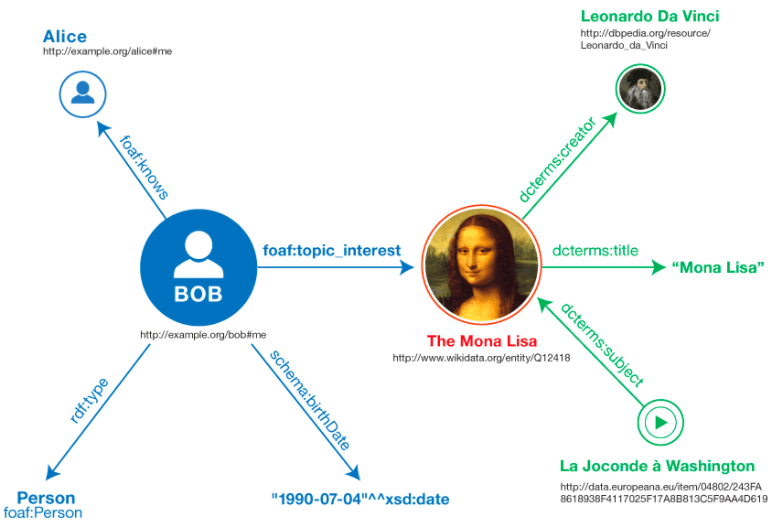
\includegraphics[width=0.87
	\textwidth,  keepaspectratio]{fig/linkedData}
	\caption{Esempio di dati rappresentati in {\tt RDF}}
	\label{fig:linkedData}
\end{figure}

\medskip

Questa modalità di rappresentare i dati viene chiamata anche {\tt Linked Data}, poiché {\tt oggetti} o {\tt classi} appartenti a {\tt vocabolari} differenti, possono essere facilmente connessi tra loro con il fine di rappresentare strutture di dati più complesse.

\medskip

I dati in {\tt RDF} possono essere espressi tramite diverse sintassi; quella mostrata in questa tesi e utilizzata da {\tt Solid}, prende il nome di {\tt Turtle} ("Terse RDF Triple Language"); i file {\tt Turtle} utilizzano il formato {\tt .ttl}. Alcuni dei possibili tipi di dati salvabili in un {\tt Pod} tramite {\tt Turtle} sono: {\tt Url, Boolean, Date, Decimal, Integer, String} e altri.

\bigskip

\section{Struttura di un Pod}

\medskip 

Per poter comprendere appieno il funzionamento dell'applicazione creata come progetto di tesi, è necessario conoscere come è strutturato un {\tt Pod}. Innanzitutto un {\tt Pod} è formato da {\tt containers} e da {\tt risorse}: i {\tt containers} sono degli oggetti simili a delle cartelle che contengono le {\tt risorse};
il {\tt Pod} di un utente è infatti gestito in maniera simile ad un file system di un calcolatore. Le {\tt risorse} invece vanno intese come l'insieme di oggetti e delle loro proprietà, espresse in linguaggio {\tt RDF}, che servono a descrivere la informazioni contenute nel {\tt Pod}.

\medskip

Per esempio all'interno di ciascun {\tt Pod} è presente il {\tt container} {\tt profile}, il quale contiene le informazioni relative al profilo dell'utente possessore del {\tt Pod}.

\medskip

\href{https://carlotosoni99.inrupt.net/profile/}{$https://carlotosoni99.inrupt.net/profile/$}

\medskip

Visitando questo link è possibile vedere che all'interno di questo {\tt container} si trova una risorsa chiamata {\tt card}, nella quale sono presenti tutte le informazioni di interesse dell'utente. In particolare in questo {\tt dataset} è collocato un oggetto avente {\tt IRI} pari a:

\medskip

\href{https://carlotosoni99.inrupt.net/profile/card\#me}{$https://carlotosoni99.inrupt.net/profile/card\#me$}

\medskip

Questo oggetto serve a rappresentare tutte le informazioni più rilevanti riguardanti il {\tt Pod} e il suo utente; da notare che l'{\tt URL} di questo oggetto corrisponde con la {\tt webId} dell'utente stesso. Ogni utente può liberamente leggere il {\tt SolidDataset} {\tt card} anche senza essersi autenticato con il {\tt Solid Identity Provider}.

\medskip

All'interno di un {\tt Pod} esistono altri {\tt containers} e altre {\tt risorse}, oltre a quelli già elencati, che servono a memorizzare differenti tipi di informazioni. In generale, comunque, ogni utente avente diritto di scrittura è libero di aggiungere {\tt containers} e {\tt risorse} all'interno di un {\tt Pod}, per poterlo gestire in base alle proprie necessità.

\medskip

L'applicazione \href{https://podbrowser.inrupt.com/}{$https://podbrowser.inrupt.com/$} sviluppata da {\tt Inrupt}, società fondata da Berners-Lee, permette di vedere il contenuto del proprio {\tt Pod} in maniera user friendly, potendo visualizzare la struttura di {\tt containers} e le rispettive {\tt risorse} al loro interno.

\bigskip

\section{Tipologie di permesso in Solid}

\medskip

In {\tt Solid} non tutti gli utenti sono autorizzati a modificare le risorse contenute all'interno di un {\tt Pod}; il {\tt vocabolario} {\tt ACL} (access control list), già enunciato, viene utilizzato per determinare se un utente è autorizzato o meno a compiere una determinata operazione. Il vocabolario {\tt ACL} descrive quattro diversi tipologie di permessi:

\medskip

\begin{itemize}
	\item {\tt Read}: permesso in lettura su una {\tt risorsa}.
	\item {\tt Append}: permesso di aggiungere ulteriori informazioni ad una {\tt risorsa} già\\ esistente, senza poterla eliminare.
	\item {\tt Write}: permesso di eseguire operazioni in scrittura su una {\tt risorsa}, potendo creare, modificare o eliminare una determinata {\tt risorsa} nel {\tt Pod}.
	\item {\tt Control}: permesso di eseguire operazioni in lettura e scrittura su un file {\tt ACL} correlato con una {\tt risorsa}.
\end{itemize}

\medskip

Nel momento in cui ci si autentica nel proprio {\tt Pod} tramite un'applicazione {\tt Solid} per la prima volta, viene data all'utente la possibilità di scegliere quali debbano essere i permessi di tale applicazione sulle {\tt risorse} presenti all'interno del proprio {\tt Pod}. Tali permessi possono essere eventualmente revocati in un secondo momento.

\medskip

Inoltre modificando le {\tt risorse ACL} presenti all'interno del proprio {\tt Pod}, è possibile andare a personalizzare le tipologie di permesso dell'applicazione sulle singole {\tt risorse} presenti.
\medskip

Per ulteriori chiarimenti riguardanti il sistema di autorizzazione usato da {\tt Solid} è possibile leggere il documento {\tt Web Access Control} \cite{wac}.

\bigskip

\section{Autenticazione in Solid}

\medskip

Spesso le applicazioni {\tt Solid} necessitano di autenticarsi con il/i {\tt Solid Identity Provider} appartente/i all'/agli utente/i in questione; tale operazione è spesso necessaria per poter ottenere i permessi necessari all'applicazione per poter interagire con le {\tt risorse} contenute all'interno dei {\tt Pod}. A seguito dell'operazione di autenticazione, le applicazioni {\tt Solid} vengono quindi autorizzate dal {\tt Solid Identity Provider} ad eseguire alcune operazioni sui dati dell'utente in base alle tipologie di permesso concesse.

\medskip

{\tt Inrupt} mette a disposizione una serie di librerie che permettono di autenticarsi con il proprio {\tt Solid Identity Provider} da Browser oppure tramite {\tt Node.js}.

\medskip

Utilizzando le librerie {\tt Inrupt} la procedura di autenticazione è relativamente semplice da eseguire: è necessario innanzitutto indicare il proprio {\tt Solid Identity Provider}, dopodiché l'utente viene indirizzato presso di questo per completare l'operazione di autenticazione con i propri dati (username e password); una volta terminata questa operazione l'utente è reindirizzato all'applicazione che stava utilizzando.

\medskip

Per ulteriori informazioni riguardanti il processo di autenticazione in {\tt Solid}, è possibile visitare la seguente pagina:\\
\href{https://solid.github.io/authentication-panel/solid-oidc/}{https://solid.github.io/authentication-panel/solid-oidc/}.

\bigskip

\section{Ulteriori chiarimenti riguardo la tecnologia Solid}

\bigskip

Qui di seguito vengono ora espressi nel dettaglio ulteriori concetti relativi alla tecnologia {\tt Solid}, i quali sono utili per comprendere in maniera più approfondita il progetto.

\bigskip

{\tt Solid} è una tecnologia che non si pone l'obiettivo di reinventare il web, ma che mira ad aggiungere a questo alcune caratteristiche, come la presenza di un sistema di identificazione per evitare di dover creare un account su ogni piattaforma presente all'interno della rete, come Facebook, Twitter, Google e molte altre. Obiettivo di {\tt Solid} è inoltre la possibilità di permettere ai vari social media, di condividere i dati relativi ai singoli utenti, indipendente dal tipo di social media utilizzato. Le applicazioni {\tt Solid} possono funzionare correttamente anche senza salvare in database locali alcun dato relativo ai singoli utenti; infatti come già detto, tutti i dati vengono salvati all'interno dei {\tt Pod} degli utenti. {\tt Solid} inoltre mette a disposizione dell'utente la possibilità di ospitare il proprio {\tt Pod} all'interno del suo hard disk o server, senza doversi affidare ad un {\tt Solid Identity Provider}. É anche possibile, quindi, divenire un piccolo {\tt Pod Provider} o {\tt Identity Provider}, con il fine di ospitare i {\tt Pod} appartenti, per esempio, alla propria famiglia, o ai membri dell'organizzazione di cui si fa parte. Un utente può inoltre possedere più di un {\tt Pod} contemporaneamente e salvare su ognuno di essi differenti tipologie di dati in relazione alle proprie necessità; inoltre sussiste la possibilità di cambiare {\tt Pod Provider} in un secondo momento, recuperando i dati presenti all'interno del {\tt Pod}.

\bigskip
\medskip

Riguardo al sistema di identificazione presente in {\tt Solid}, una {\tt webId} non deve\\ necessariamente essere usata per identificare una persona fisica, bensì può riferirsi anche a organizzazioni, compagnie, famiglie, team o, più generalmente, a qualsiasi gruppo di persone.

\bigskip
\medskip

Per quanto concerne la sicurezza dei dati salvati all'interno del proprio {\tt Pod} è bene fare alcune precisazioni. Innanzitutto il livello di sicurezza dei propri dati dipende dal {\tt Pod Provider} utilizzato; i {\tt Pod Provider}, in generale, non hanno vincoli riguardanti la crittografia utilizzata per criptare i dati contenuti all'interno del {\tt Pod}. L'utente ha il compito di scegliere un {\tt Pod Provider} che cripti i propri dati adeguatamente se la sicurezza di questi è importante per lui. Infine, poiché {\tt Solid} non prevede che i dati relativi ad un utente debbano essere necessariamente salvati all'interno di un singolo luogo, essendo possibile utilizzare più di un {\tt Pod} per la memorizzazione delle proprie informazioni, {\tt Solid} non rende gli utenti maggiormente vulnerabili da parte di attacchi informatici. A tal proposito è necessario considerare anche che attacchi informatici da parte di hackers sono maggiormente probabili se riferiti a una singola fonte di dati di molte persone, piuttosto che a livello individuale.



\bigskip
\bigskip
\bigskip
\bigskip

All'interno del sito web \href{https://solidproject.org/}{https://solidproject.org/} sono presenti ulteriori informazioni, per sviluppatori e non, riguardanti il progetto {\tt Solid}.

\bigskip

\section{Inrupt}

\medskip

{\tt Inrupt} è una società fondata da Sir Tim Berners-Lee nel 2018 per fornire strumenti atti a favorire lo sviluppo di {\tt Solid}. Secondo Berners-Lee, {\tt Inrupt} mira a "fornire energia commerciale e un ecosistema per aiutare a proteggere l'integrità e la qualità del nuovo web costruito su Solid" \cite{inrupt}.

\medskip

In particolare {\tt Inrupt} fornisce una serie di strumenti per potersi autenticare con il proprio {\tt Solid Identity Provider} e per poter aggiungere, creare, modificare e cancellare le informazioni all'interno del proprio {\tt Pod}.

\medskip

Le librerie create da {\tt Inrupt}, e usate anche nel progetto oggetto della tesi, sono:

\begin{itemize}
	\item {\tt solid-client-authn-browser}: tale libreria permette di autenticarsi con il proprio {\tt Solid Identity Provider} tramite browser.
	\item {\tt solid-client-authn-node}: questa libreria permette di autenticarsi con il proprio {\tt Solid Identity Provider} tramite Node.js.
	\item {\tt solid-ui-react}: mette a disposizione componenti per applicazioni in React per potersi autenticare con il proprio {\tt Solid Identity Provider} e per poter leggere e scrivere le informazioni contenute all'interno del {\tt Pod}.
	\item {\tt solid-client}: fornisce funzioni atte a eseguire ogni possibile azione all'interno del proprio {\tt Pod}, tra le quali: scaricare {\tt SolidDataset} presenti all'interno del proprio {\tt Pod}, modificare un {\tt SolidDataset} già esistente o crearne uno all'interno del proprio {\tt Pod}, caricare, modificare un {\tt oggetto} appartenente ad un determinato {\tt SolidDataset}, oppure crearne uno nuovo, leggere gli {\tt statement} di un {\tt oggetto} per poter ricavare informazioni presenti nel proprio {\tt Pod}, oppure modificare {\tt statement} già esistenti o crearne dei nuovi, leggere e scrivere {\tt risorse ACL} e utilizzare altre funzionalità.
\end{itemize}

\medskip

Le librerie messe a disposizioni da {\tt Inrupt} sono attualmente le più utilizzate per programmare applicazioni in {\tt Solid}. Oltre a questo, {\tt Inrupt} gestisce uno dei due {\tt Solid Identity Provider} più utilizzati al momento;\\
visitando il seguente URL si può accedere al sito \href{https://inrupt.net/}{https://inrupt.net/} per potersi\\registrare con il {\tt Solid Identity Provider} e creare un proprio {\tt Pod}.

\medskip

Per leggere la documentazione relativa alle librerie sopra enunciate è possibile\\visitare i seguenti URL:

{\tt solid-client-authn-browser} e {\tt solid-client-authn-node}:\\ \href{https://docs.inrupt.com/developer-tools/javascript/client-libraries/authentication/}{https://docs.inrupt.com/developer-tools/javascript/client-libraries/authentication/}\\
{\tt solid-ui-react}:\\ \href{https://solid-ui-react.docs.inrupt.com/?path=/story/intro--page}{https://solid-ui-react.docs.inrupt.com/?path=/story/intro--page} \\
{\tt solid-client}:\\
\href{https://docs.inrupt.com/developer-tools/javascript/client-libraries/tutorial/read-write-data/}{https://docs.inrupt.com/developer-tools/javascript/client-libraries/tutorial/read-write-data/} e\\
\href{https://docs.inrupt.com/developer-tools/api/javascript/solid-client/}{https://docs.inrupt.com/developer-tools/api/javascript/solid-client/}

\medskip

\section{React}

\medskip

{\tt React} è una libreria {\tt open-source}, {\tt front-end}, {\tt JavaScript}, finalizzata alla creazione di interfacce utente ed attualmente molto conosciuta e usata. Vengono qui elencate le caratteristiche principali di {\tt React}:

\medskip 

\begin{itemize}
	\item Permette di creare interfacce grafiche in maniera semplificata. Le interfacce sono progettate per ogni stato dell'applicazione; ad ogni cambio di stato {\tt React} aggiorna solo le parti delle UI che dipendono da tali dati.
	\item Agevola la creazione di interfacce grafiche complesse, permettendo di creare componenti in isolamento e ricomponibili per formare UI complesse.
	\item {\tt React} non è dipendente da altre tecnologie: in questo modo si possono sviluppare nuove funzionalità in {\tt React} senza dover riscrivere qualsiasi codice già esistente.
\end{itemize}

\medskip

{\tt JSX} è la sintassi che {\tt React} utilizza per descrivere l'aspetto delle interfacce grafiche. Comunque l'utilizzo di {\tt JSX}, pur essendo raccomandato, risulta opzionale e non richiesto per programmare in {\tt React}. {\tt JSX} va inteso come un'estensione della sintassi di {\tt Javascript}, riprendendo le proprie caratteristiche sia da {\tt Javascript} stesso che da {\tt HTML}.

\bigskip

L'applicazione {\tt my-solid-blog} è stata sviluppata utilizzando {\tt React} e, in particolare, il comando {\tt create-react-app} di {\tt npx}, il quale permette di creare applicazioni in {\tt React} single-page. {\tt create-react-app} crea autonomamente un ambiente di sviluppo che consente di utilizzare le caratteristiche più recenti di {\tt JavaScript}, utilizzando, per esempio, {\tt Babel} e {\tt webpack}.

\bigskip

Le motivazioni che hanno portato a sviluppare {\tt my-solid-blog} in {\tt React} sono principalmente due: la prima è che la libreria {\tt solid-ui-react} di {\tt Inrupt} permette ad applicazioni in {\tt React} di gestire alcune operazioni in {\tt Solid}, come l'autenticazione con {\tt Solid Identity Provider}, in maniera semplice e intuitiva; il secondo motivo riguarda la semplicità con cui {\tt React} permette agli sviluppatori di creare e gestire interfacce grafiche. Per renderizzare le proprie interfacce grafiche, l'applicazione {\tt my-solid-blog} utilizza la sintassi {\tt JSX}. Le applicazioni {\tt React} create tramite comando {\tt create-react-app} possono essere avviate in {\tt development mode} utilizzando il comando {\tt npm start}.

\bigskip

Per ulteriori informazioni relative alla libreria {\tt React} è possibile visitare il sito web:

\smallskip

\href{https://it.reactjs.org/}{https://it.reactjs.org/}.

\bigskip

\section{Bulma}

\medskip

{\tt Bulma} è un framework {\tt CSS} {\tt open source} che si è particolarmente diffuso negli ultimi anni, raggiungendo 40.000 stelle su {\tt GitHub}. È caratterizzato da una sintassi semplice che permette di importare nei propri progetti vari componenti predefiniti; {\tt Bulma} presenta un design minimalista e unico nel suo genere, capace di rendere maggiormente accattivamente una pagina web.

\bigskip

Il framework {\tt Bulma} è stato scelto per gestire il layout dell'applicazione\\{\tt my-solid-blog} per la sua semplicità, per il suo design e per la compatibilità con la libreria {\tt React}.

\medskip

Visitando il seguente URL è possibile leggere la documentazione relativa a {\tt Bulma}:

\smallskip

\href{https://bulma.io/}{https://bulma.io/}

\bigskip

\section{Node.js}

\medskip

{\tt Node.js} è un {\tt runtime system} {\tt open source} multipiattaforma {\tt orientato agli eventi}. Quando è stato introdotto, {\tt Node.js} ha consentito l'esecuzione di codice {\tt JavaScript} da {\tt lato server}; precedentemente {\tt JavaScript} era stato utilizzato principalmente da {\tt lato Client}. Data la sua enorme potenzialità, {\tt Node.js} è attualmente una delle tecnologie più richieste sul mercato del lavoro.

\bigskip

All'interno di questo progetto {\tt Node.js} è stato utlizzato per sviluppare l'applicazione {\tt blog-validator}, con lo scopo di effettuare alcuni controlli sui dati presenti nel {\tt Pod}. Tale server si occupa infatti di verificare l'autenticità dei dati mostrati dall'applicazione {\tt my-solid-blog} su richiesta dell'utente.

\clearpage

\section{Altri strumenti utilizzati}

\bigskip

\textbf{Axios}

\bigskip

{\tt Axios} è una libreria che permette di inviare richieste {\tt HTTP} da browser o da {\tt Node.js}. Tale libreria è stata utilizzata per permettere la trasmissione di informazioni tra l'applicazione {\tt my-solid-blog} e il server {\tt Node.js}, con il fine di comunicare al server alcune informazioni relative ai contenuti mostrati all'interno dell'applicazione stessa.

\smallskip

\href{https://github.com/axios/axios}{https://github.com/axios/axios}

\bigskip

\textbf{vocab-common-rdf e rdf-namespaces}

\bigskip

Queste due librerie di {\tt JavaScript} contengono degli pseudonimi per i vocabolari {\tt RDF} più utilizzati, permettendo di utilizzare {\tt proprietà} e {\tt classi} di alcuni vocabolari {\tt RDF} in maniera semplificata e snellendo il codice dell'applicazione.

\medskip

Ad esempio la libreria {\tt rdf-namespaces} permette di utilizzare la proprietà {\tt type} del vocabolario {\tt http://www.w3.org/1999/02/22-rdf-syntax-ns} semplicemente scrivendo {\tt rdf.type}, anziché\\{\tt http://www.w3.org/1999/02/22-rdf-syntax-ns\#type}.

\medskip

Tale proprietà, fondamentale nel linguaggio {\tt RDF}, è utilizzata per indicare che una {\tt risorsa} è un'instanza di una {\tt classe}.

\clearpage
\chapter{Motivazioni del progetto}

\medskip

\section{L'evoluzione del World Wide Web}

\medskip

\begin{figure}[ht]
	\centering
	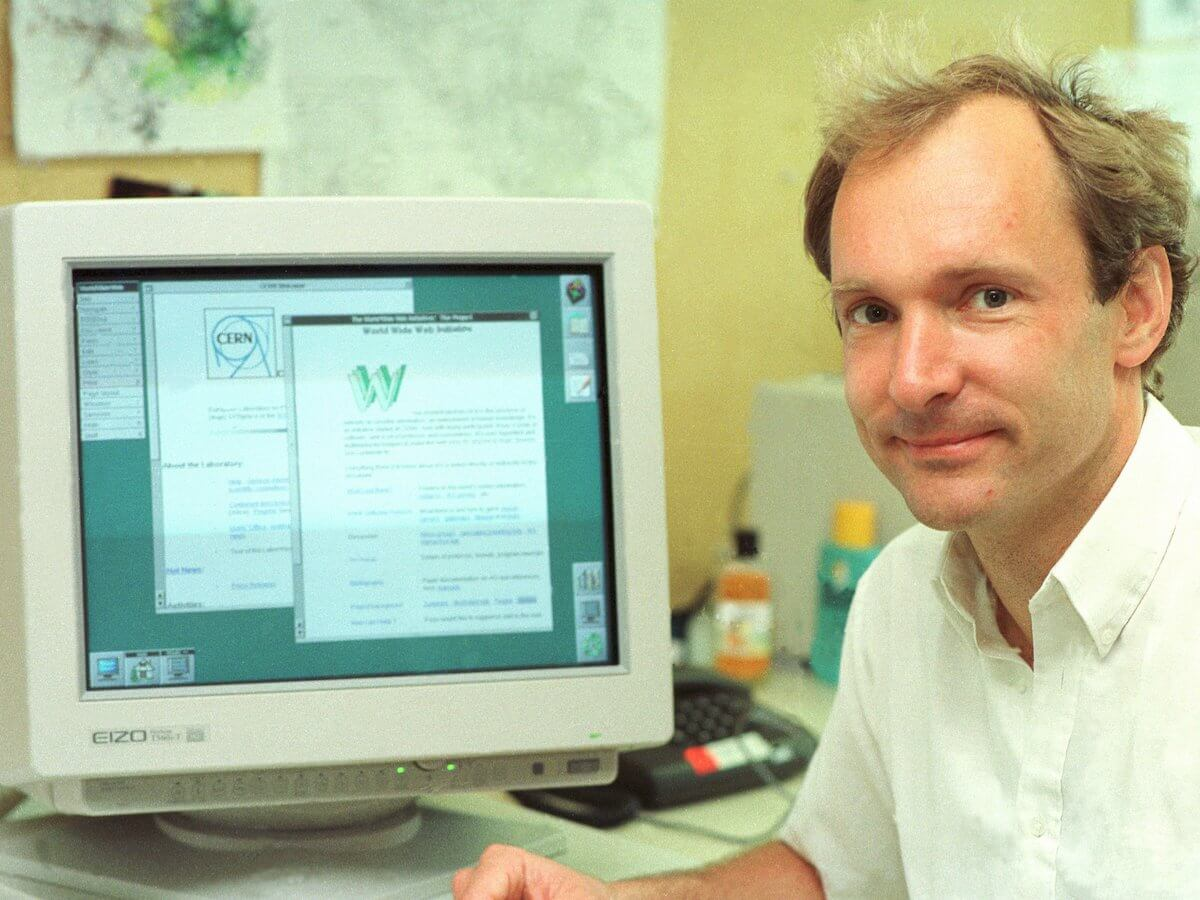
\includegraphics[width=0.87
	\textwidth,  keepaspectratio]{fig/Berners-Lee}
	\caption{Sir Tim Berners-lee, fondatore del {\tt World Wide Web}, davanti al primo prototipo di browser.}
	\label{fig:bernersLee}
\end{figure}

\medskip 

Sir Tim Berners-Lee, fondatore del {\tt World Wide Web} e del progetto {\tt Solid}, insignito del premio Turing nel 2016, con il passare degli anni fu mosso da una crescente preoccupazione relativa al modo con cui la sua creazione, il {\tt WWW}, si era evoluta. Con il passare del tempo iniziò a dubitare del reale beneficio apportato da questa tecnologia alla società umana \cite{sciencefocus}.

\bigskip

Nella visione di Berners-Lee, il {\tt World Wide Web} sarebbe dovuto essere un luogo in cui tutti gli utenti, attraverso un meccanismo di autorizzazioni, avrebbero potuto collaborare per creare nuovi contenuti sulla rete. Infatti, il primo browser della storia, sviluppato nel {\tt CERN} di Ginevra, era stato progettato per essere anche un editor, con il fine di permettere uno scambio di dati in maniera decentralizzata tra utenti. Tuttavia la prima versione di browser che rese il web popolare tagliò questa funzionalità, poiché ritenuta troppo difficile da implementare.  

\bigskip
\bigskip

Berners-Lee, il 12 marzo 2017, in occasione del ventottesimo compleanno di internet, delineò i tre principali problemi principali relativi alla sua creazione \cite{worldwideweb}:

\bigskip
\bigskip

\textbf{"We’ve lost control of our personal data"}. Gli utenti di Internet accettano di utilizzare servizi gratuitamente in cambio della cessione dei loro dati personali; questo ha portato le grandi multinazionali, come i più importanti social network, a collezionare i dati dei loro utenti per fini personali. Società e governi hanno iniziato a osservare i movimenti online degli tali utenti, portando, ad esempio, all'arresto e all'uccisione di alcuni cittadini in Paesi vittime di regimi dittatoriali. \cite{bloggers}

\bigskip
\bigskip

\textbf{"It’s too easy for misinformation to spread on the web"}. Tramite i dati raccolti dagli utenti, attraverso l'utilizzo di appositi algoritmi, i social network possono mostrare contenuti in base ai loro interessi, inviando loro link ad altri siti web. Tali siti spesso risultano essere fonti di disinformazione o di fake news e mostrano all'utente contenuti in base alle sue credenze e ai suoi pregiudizi in modo da condizionarne le idee \cite{nyt}\label{key}.

\bigskip
\bigskip

\textbf{"Political advertising online needs transparency and understanding"}. Berners-Lee ha infine evidenziato i problemi connessi con l'industria delle publicità politiche. Tramite i dati degli utenti, i quali vengono continuamente raccolti dai social network, vengono create pubblicità individuali rivolte ai singoli, in base ai loro dati. É stato stimato da una fonte \cite{guardian} che, durante le elezioni presidenziali degli Stati Uniti d'America del 2016, siano state create ogni giorno circa 50.000 variazioni di pubblicità di natura politica con il fine di renderle più adatte ai singoli utenti. Berners-Lee ritenne che vi fossero molti indizi sulla non eticità di tali pubblicità.

\bigskip
\bigskip

Le preoccupazioni di Berners-Lee si sono ulteriormente acuite a seguito dello scandalo Facebook-Cambridge Analytica, avvenuto nel 2018. Tale scandalo mise in evidenza che il noto social network Facebook aveva raccolto dati di 87 milioni di utenti senza il loro consenso per scopi di propaganda politica \cite{facebook}. 

\bigskip

\section{Nascita del progetto Solid}

\medskip

Queste considerazioni hanno portato alla nascita del progetto {\tt Solid} da parte di {\tt Berners-Lee}. Egli mira a superare le problematiche elencate rendendo gli utenti i veri proprietari del web, ridecentralizzandolo, come quando lo aveva originariamente creato \cite{techchahiye}.

\medskip

Il progetto nasce già nel 2015 in collaborazione con il {\tt MIT}; allo sviluppo di questa tecnologia hanno collaborato anche l'Università di Oxford e l'Istituto di Ricerca Informatica del Qatar. Nel 2018 Berners-Lee si prende un anno sabbatico dal progetto per fondare la società {\tt Inrupt}, già menzionata nel capitolo 2, con il fine di mettere a disposizione degli sviluppatori strumenti per poter interagire con {\tt Solid}.

\medskip

Come in parte già descritto, {\tt Solid} mira a risolvere i problemi evidenziati da Berners-Lee, cambiando il modello attuale di consegna dei propri dati ai giganti informatici in cambio dell'accesso ad alcuni servizi, poiché tale modello penalizza gli utenti del web, privandoli della loro privacy. {\tt Solid} mira ad evolvere il web riequilibrandolo, dando ad ognuno il completo controllo dei propri dati, personali e non, in modo innovativo. Berners-Lee è fermamente convinto riguardo la necessarietà di {\tt Solid} per poter modificare il web, sostenendo che, tramite questa tecnologia le persone riusciranno a riprendersi il loro potere dalle grandi corporazioni. A tal proposito Berners-Lee ha dichiarato: "Non stiamo chiedendo a Facebook o a Google se introdurre o meno un completo cambiamento (sul web) che porterà a capovolgere completamente il loro modello di business, non stiamo chiedendo a loro permessi" \cite{fastcompany}.


\bigskip

\section{Nascita del sistema SADeB}

\medskip

Il sistema {\tt SADeB} (Solid Authenticity Decentralized Blog) nasce con l'intento di mettere in evidenza le potenzialità della tecnologia {\tt Solid}, mostrando le differenze tra l'applicazione {\tt Solid} {\tt my-solid-blog} e un normale social network.

\medskip

Come già descritto, le applicazioni {\tt Solid} sono totalmente svincolate dai dati che mostrano all'utente con cui interagiscono; ciò permette all'utente stesso di controllare i propri dati in maniera diretta, di comprendere chi li sta utilizzando e di permettere che questi vengano riutilizzati da più applicazioni differenti in base alle sue necessità. 

\medskip

La decentralizzazione effettuata da {\tt Solid} permette, inoltre, di tutelare l'utente che utilizza tali applicazioni, arginando in parte il problema relativo alla diffusione di disinformazione, evidenziato anche da Berners-Lee stesso \cite{worldwideweb}. Infatti, tramite {\tt Solid}, è possibile implementare in maniera semplice ed efficiente dei controlli sull'autenticità dei dati mostrati all'utente. L'applicazione {\tt blog-validator}, facente parte del sistema {\tt SADeB}, si occupa, infatti, di controllare che l'applicazione {\tt my-solid-blog} non abbia volontariamente modificato i dati contenuti all'interno del {\tt Pod} dell'utente, con il fine di diffondere informazioni false. {\tt blog-validator} si occupa quindi di comparare i dati visualizzati da {\tt my-solid-blog} con quelli realmente presenti all'interno del {\tt Pod} dell'utente, indicando, eventualmente a quest'ultimo, se tali dati siano stati modificati. {\tt blog-validator} è un'applicazione esterna e svincolata da {\tt my-solid-blog}, creata per poter essere utilizzata, apportando alcune modifiche al codice in base alle necessità, non solo da {\tt my-solid-blog}, ma anche da altre possibili applicazioni decentralizzate, per dare garanzie ai loro utenti riguardo la validità delle informazione loro mostrate.

\clearpage

\chapter{Il problema affrontato}

\medskip

L'obiettivo del presente elaborato è mostrare il funzionamento di un blog decentralizzato sviluppato tramite tecnologia {\tt Solid}, mettendo in evidenza i benefici che un'applicazione {\tt Solid} può apportare all'utente.

\medskip

Il progetto è composto da due applicazioni differenti e svincolate tra di loro. La prima è chiamata {\tt my-solid-blog}; tale applicazione offre due differenti tipologie di servizi: la prima consiste nel permettere la creazione di un proprio blog, salvando tutte le informazioni di interesse all'interno del suo {\tt Pod}. In questo caso, per poter ottenere il diritto in scrittura sui dati presenti all'interno del {\tt Pod}, l'applicazione richiede preventivamente all'utente di autenticarsi con il proprio {\tt Solid Idenitity Provider}; il secondo servizio implementato in {\tt my-solid-blog} consiste nel permettere la lettura di blog di altre persone una volta conosciuta la loro {\tt webId}. Per questa seconda funzionalità la procedura di autenticazione  con il proprio {\tt Solid Identity Provider} non è richiesta.

\medskip

La seconda applicazione trattata in questo elaborato di tesi, chiamata {\tt blog-validator}, permette, su richiesta dell'utente, di effettuare controlli riguardo l'autenticità dei dati mostrati da {\tt my-solid-blog}. Tale applicazione ha lo scopo di evidenziare la semplicità con cui un'operazione di questo tipo può essere implementata in {\tt Solid}.

\bigskip

\section{Obiettivi del progetto}

\medskip

Il sistema {\tt SADeB} consiste di due applicazioni differenti: {\tt my-solid-blog} e {\tt blog-validator}. Vengono ora elencate le specifiche relative all'applicazione\\{\tt my-solid-blog}.

\medskip

\begin{itemize}
	\item L'applicazione {\tt my-solid-blog} deve essere completamente decentralizzata, rispettando i principi della tecnologia {\tt Solid}.
	\item Una volta avviata l'applicazione, l'utente deve poter scegliere la modalità con cui interagire con l'app, indicando se vuole autenticarsi con il proprio {\tt Solid Identity Provider} e modificare, creare ed eliminare i dati presenti all'interno del proprio blog, oppure se inserire la {\tt webId} di un altro utente per visualizzare il blog di quest'ultimo.
	\item L'applicazione deve implementare un meccanismo di autenticazione con il server {\tt Solid}, sfruttando le librerie messe a disposizione da {\tt Inrupt}.
	\item Una volta che l'utente si è autenticato con il proprio {\tt Solid Identity Provider}, l'applicazione {\tt my-solid-blog} deve poter controllare se esiste all'interno del {\tt Pod} dell'utente un {\tt SolidDataset} relativo al blog. In questo caso, {\tt my-solid-blog} deve caricare tale {\tt SolidDataset} per poter leggere e modificare i dati contenuti in esso. Altrimenti l'applicazione deve creare tale dataset all'interno del {\tt Pod} dell'utente. Il nome del {\tt SolidDataset} utilizzato dall'applicazione è {\tt articlelist.ttl}.
	\item I dati contenuti all'interno del {\tt SolidDataset} {\tt articlelist.ttl} utilizzato da\\ {\tt my-solid-blog}, devono rappresentare degli articoli da pubblicare sul blog\\relativo all'utente che è proprietario del {\tt Pod}. Per poter rappresentare tali dati, l'applicazione deve far uso del vocabolario {\tt RDF} {\tt Schema}.
	\item Ogni articolo deve avere un titolo, un testo che ne rappresenti il contenuto, una data di creazione e un identificatore univoco. Ogni articolo è un oggetto e un'istanza della classe {\tt TextDigitalDocument} del vocabolario {\tt Schema}. L'applicazione deve permettere all'utente di visualizzare il titolo, il contenuto e la data di creazione di ciascun articolo presente.
	\item L'applicazione {\tt my-solid-blog} deve permettere all'utente autenticato di leggere, modificare e cancellare i dati, cioé gli articoli, presenti all'interno del {\tt SolidDataset} {\tt Articlelist.ttl}. A tal proposito {\tt my-solid-blog} deve utilizzare le librerie {\tt Inrupt} per poter svolgere queste operazioni sui dati contenuti all'interno del {\tt Pod}. 
	\item L'utente autenticato deve essere, inoltre, in grado di scrivere nuovi articoli all'interno del proprio blog.
	\item Un utente può scegliere di accedere al contenuto di un blog di un secondo utente, inserendo la sua {\tt webId} senza passare per alcun processo di autenticazione. In questo caso, se esiste il {\tt SolidDataset} {\tt articlelist.ttl} all'interno del {\tt Pod} corrispondente alla {\tt webId} inserita, l'applicazione deve permettere all'utente di visualizzare gli articoli relativi alla {\tt webId} inserita.
	\item Se l'utente accede ad un blog inserendo la {\tt webId} corrispondente al {\tt Pod} ove questo è memorizzato, senza quindi passare per un processo di autenticazione, non deve essere in grado di modificare il contenuto degli articoli all'interno di tale {\tt Pod}. Inoltre l'utente non autenticato non deve avere i permessi necessari per scrivere nuovi articoli all'interno del {\tt SolidDataset} {\tt articlelist.ttl} corrispondente alla {\tt webId} inserita.
	\item L'applicazione {\tt my-solid-blog} deve poter comunicare tramite il protocollo {\tt HTTP} con il server {\tt blog-validator}, per potergli inviare, su richiesta dell'utente, i dati necessari ad effettuare un controllo all'interno del {\tt Pod} del proprietario di questi dati. Per implementare tale funzionalità, {\tt my-solid-blog} deve renderizzare per ogni articolo un pulsante {\tt Check} per innescare tale controllo sull'autenticità dei contenuti visualizzati. Il controllo è riferito al singolo articolo selezionato, e non all'intero {\tt SolidDataset}.
	\item Ogni utente, indipendentemente dal fatto che abbia completato l'operazione di autenticazione o meno con il server {\tt Solid}, deve essere in grado di richiedere un controllo sull'autenticità dei contenuti mostrati da {\tt my-solid-blog}.
	\item L'applicazione {\tt my-solid-blog} deve mettere a disposizione un link che rimandi a {\tt blog-validator} per poter permettere a tutti gli utenti, autenticati e non, di verificare che eventuali controlli sull'autenticità dei dati effettuati siano stati eseguiti correttamente.
	\item Ogni utente deve poter visualizzare l'URL associato all'articolo che sta leggendo, ovvero l'URL ove tale risorsa è stata memorizzata.
	\item Le interfacce grafiche dell'applicazione, create tramite {\tt React}, devono essere semplici e intuitive, in modo tale da rendere l'applicazione user friendly.
\end{itemize}

\bigskip

Vengono qui di seguito elencate le specifiche relative all'applicazione {\tt blog-validator}.

\begin{itemize}
	\item Tramite il protocollo {\tt HTTP}, l'applicazione deve poter ricevere da\\{\tt my-solid-blog} le informazioni necessarie per effettuare un controllo sull'autenticità dei dati mostrati. In particolare {\tt blog-validator} si occupa di verificare che un singolo articolo, scelto dall'utente, sia effettivamente presente all'interno del {\tt Pod} dell'utente proprietario del blog. Una volta terminato tale controllo, l'applicazione {\tt blog-validator} deve inviare a {\tt my-solid-blog} l'esito del controllo stesso.
	\item I possibili esiti di un controllo sono i seguenti:
	
	\smallskip
	
	\textbf{1)} L'articolo in questione non esiste all'interno del {\tt Pod} del proprietario.\\
	\textbf{2)} L'articolo esiste, ma il contenuto risulta essere differente.\\
	\textbf{3)} L'articolo esiste e presenta lo stesso contenuto, ma la data in cui è stato pubblicato è differente.\\
	\textbf{4)} Il controllo sull'autenticità del contenuto ha dato un risultato positivo: in questo caso il server non ha rilevato alcuna anomalia.
	\item {\tt blog-validator} deve mettere a disposizione un URL per permettere all'utente di visualizzare i dati relativi ai controlli già effettuati sul {\tt Pod} di un utente. Questa funzionalità di {\tt blog-validator} serve ad assicurarsi che {\tt my-solid-blog} abbia inviato correttamente i dati relativi ai controlli effettuati, senza manometterli.
	\item {\tt blog-validator}, infine, deve poter permettere all'utente di effettuare controlli manualmente sulle risorse relative ai blog creati da {\tt my-solid-blog}; insererendo l'url del articolo che si vuole controllare e del {\tt SolidDataset} dove è memorizzato, {\tt blog-validator} deve mostrare all'utente contenuto, titolo e data di creazione dell'articolo, nel caso in cui questo sia effettivamente presente all'interno del {\tt Pod}.
\end{itemize}

\bigskip

\section{Modalità di accesso ai dati contenuti nel Pod}

\medskip

Nel corso dello svolgimento del progetto si è rivelata fondamentale la comprensione delle modalità con cui un'applicazione {\tt Solid} debba accedere ai dati contenuti all'interno del {\tt Pod}. Innanzitutto entrambe le applicazioni, {\tt my-solid-blog} e {\tt blog-validator}, utilizzano la libreria {\tt Inrupt} {\tt solid-client} per poter interagire con tali dati; la libreria mette a disposizione una serie di funzioni per poter scaricare {\tt SolidDataset} e per poter modificare gli oggetti al suo interno. 

\bigskip

Vengono qui mostrate le funzioni più importanti contenute in tale libreria:

\bigskip
\medskip

$getSolidDataset(url, options?): Promise<SolidDataset \& WithServerResourceInfo>$

\bigskip

Funzione che restituisce una {\tt promessa} che si risolve nel {\tt SolidDataset} corrispondente all'URL indicato; l'utente deve possedere il diritto in lettura su tale risorsa per poter caricare tale {\tt SolidDataset}. A tal scopo, se necessario, può passare alla funzione i dati relativi alla sessione di autenticazione con il {\tt Solid Identity Provider}, per poter acquisire tale diritto in lettura.

\bigskip
\medskip

$saveSolidDatasetAt<Dataset>(url, solidDataset, options?): Promise<Dataset\\ \& WithServerResourceInfo \& WithChangeLog>$

\bigskip

Tale funzione permette di salvare un determinato {\tt SolidDataset} all'interno dell'URL specificato; si possono passare a questa funzione anche i dati relativi alla sessione di autenticazione con il {\tt Solid Identity Provider} per acquisire diritto in scrittura sulle risorse del {\tt Pod}. Il possesso del diritto in scrittura è una condizione necessaria per poter utilizzare tale funzione. Restituisce una {\tt promessa} che si risolve nel nuovo {\tt SolidDataset} presente a seguito dell'esecuzione di questa funzione. Tale funzione, inoltre, può essere utilizzata per tenere traccia dei cambiamenti apportati all'interno di tale {\tt SolidDataset}.

\bigskip
\medskip

$createSolidDataset(): SolidDataset$

\bigskip

Permette di creare un nuovo {\tt SolidDataset}.

\bigskip
\medskip

$getThing(solidDataset, thingUrl, options?): ThingPersisted | null$

\bigskip

Ritorna un oggetto presente all'interno di un {\tt SolidDataset}, è necessario passare a tale funzione il {\tt SolidDataset} che contiene tale oggetto e l'URL relativo all'oggetto che si vuole ottenere. La funzione ritorna il valore {\tt null} se l'oggetto specificato non esiste.

\medskip
\bigskip

$getThingAll(solidDataset, options?): Thing[]$

\bigskip

Ritorna un array contenente tutti gli oggetti presenti all'interno di un {\tt SolidDataset}.

\bigskip
\medskip

$createThing(options): ThingPersisted$

\bigskip

Crea un nuovo oggetto.

\bigskip
\medskip

$setThing<Dataset>(solidDataset, thing): Dataset \& WithChangeLog$

\bigskip

Permette di aggiungere un nuovo oggetto all'interno di un {\tt SolidDataset}, rimpiazzando evenutali precedenti instanze di tale oggetto.

\bigskip
\medskip

$removeThing<Dataset>(solidDataset, thing): Dataset \& WithChangeLog$

\bigskip

Rimuove un oggetto contenuto all'interno di un {\tt SolidDataset}.

\bigskip
\medskip

$asUrl(thing, baseUrl): UrlString$

\bigskip

Restituisce l'URL dell'oggetto passato come parametro.

\bigskip
\medskip

$getUrl(thing, property): UrlString | null$

\bigskip

Permette di restituire l'oggetto di uno {\tt statement} contenuto all'interno di un oggetto. È necessario passare a tale funzione l'oggetto e il predicato di tale {\tt risorsa}, cioè il soggetto e il predicato dello {\tt statement} {\tt RDF}. Restituisce il valore {\tt null} se tale {\tt risorsa} non esiste o se il tipo della {\tt risorsa} non è URL. Se esistono più {\tt risorse} di tipo URL corrispondenti a tale predicato, la funzione restituisce un URL fra quelli presenti.

\bigskip
\medskip

$getUrlAll(thing, property): UrlString[]$

\bigskip

Restituisce tutti i valori URL relativi alla proprietà di una {\tt risorsa}.

\bigskip

Esistono inoltre funzioni simili per poter ottenere differenti tipologie di dati, come ad esempio: {\tt string, boolean, decimal, integer} e altre ancora.

\medskip
\bigskip 

$addUrl<T>(thing, property, value): T$

\bigskip

Crea un nuovo oggetto con un URL aggiunto come proprietà; eventuali altri valori relativi a tale proprietà non vengono modificati.

\bigskip

Esistono funzioni simili per poter aggiungere proprietà relative ad altre tipologie di dati, come per esempio: {\tt string, boolean, decimal, integer} e altre.

\medskip
\bigskip

$setUrl<T>(thing, property, value): T$

\bigskip

Crea un nuovo oggetto con gli esistenti valori relativi ad una proprietà rimpiazzati con l'URL passato come parametro.

\bigskip

Esistono funzioni simili per poter sostituire proprietà relative ad altre tipologie di dati, come ad esempio: {\tt string, boolean, decimal, integer} e altre.

\bigskip
\medskip

Per accedere ad alcuni dati relativi alle informazioni sul profilo dell'utente sono stati utilizzati anche i componenti della libreria {\tt Inrupt} {\tt solid-ui-react} $<CombinedDataProvider>$ e $<Text>$.

\bigskip

\section{Modalità di autenticazione con il Solid Identity Provider}

\medskip

Come già accennato riguardo alle specifiche relative all'applicazione {\tt my-solid-blog}, l'applicazione in questione deve poter permettere ai propri utenti di autenticarsi con il proprio {\tt Solid Indentity Provider} per modificare il proprio blog. Per implementare questa funzionalità è stata utilizzata la libreria {\tt Inrupt} {\tt solid-ui-react}, la quale mette a disposizione componenti {\tt React} per autenticarsi e per leggere/scrivere dati.

\bigskip

Vengono ora elencati i componenti appartenenti a questa libreria usati per implementare tale funzionalità:

\bigskip
\medskip

$<SessionProvider>$

\bigskip

Tale componente è usato per avvolgere la propria applicazione; è necessario passare al compomente una {\tt sessionId} universalmente unica. La {\tt sessionId} utilizzata nel caso dell'applicazione {\tt my-solid-blog} è {\tt my-solid-blog}. Tale componente permette di utilizzare all'interno del progetto il componente $<LoginButton>$.

\bigskip
\medskip

$<LoginButton>$

\bigskip

Permette di autenticarsi con il proprio {\tt Solid Identity Provider}, avviando quindi il procedimento di autenticazione descritto all'interno del capitolo 2. È necessario passare a tale componente le seguenti informazioni:

\begin{itemize}
	\item {\tt oidcIssuer}: in questo campo va indicato l'URL del {\tt Solid Identity Provider} con il quale ci si vuole autenticare, come per esempio {\tt https://inrupt.net/}.
	\item {\tt redirectUrl}: indica l'URL sul quale l'utente viene reindirizzato a seguito del processo di autenticazione. Poiché l'applicazione {\tt my-solid-blog} è di tipo single-page e utilizza la porta 3000, il {\tt redirectUrl} usato è pari a {\tt http://localhost:3000/}.
	\item {\tt authOptions}: opzionale, serve ad indicare informazioni aggiuntive relative alla sessione di autenticazione. {\tt my-solid-blog} utilizza tale attributo per indicare il nome dell'applicazione che si sta autenticando con il server {\tt Solid}, che è semplicemente {\tt my-solid-blog}.
\end{itemize}

\bigskip
\medskip

$useSession()$

\bigskip

Funzione contenuta all'interno della libreria {\tt solid-ui-react}, restituisce dati relativi alla sessione di autenticazione; il codice sotto indicato consente di raccogliere tali dati.

\bigskip

{\tt const { session } = useSession();}

\bigskip

L'oggetto {\tt session} contiene quindi dati relativi alla propria sessione di autenticazione, come ad esempio:

\begin{itemize}
	\item {\tt session.info.webId}: contiene la {\tt webId} dell'utente autenticato.
	\item {\tt session.info.isLoggedIn}: proprietà pari a {\tt true} se l'utente ha completato il processo di autenticazione ed è attualmente loggato con il proprio {\tt Solid Identity Provider}, altrimenti tale proprietà è pari a {\tt false}.
	\item {\tt session.fetch}: metodo usato per interagire con i dati contenuti all'interno del {\tt Pod}, usando le informazioni relative al login dell'utente. Tale funzione può essere passata come metodo alle funzioni {\tt getSolidDatasetAt} e {\tt saveSolidDatasetAt} per ottenere i permessi necessari a completare tali operazioni sui dati all'interno del {\tt Pod}.
\end{itemize}

\clearpage


\chapter{Il sistema SADeB}

\medskip

Come già precedentemente indicato, il sistema {\tt SADeB} (Solid Authenticity Decentralized Blog), è formato dalle due applicazioni {\tt my-solid-blog} e {\tt blog-validator}.

\bigskip

\textbf{Vengono ora descritti nel dettaglio l'implementazione e le modalità di funzionamento dell'applicazione my-solid-blog.}

\bigskip

\section{Directory e file presenti in my-solid-blog}

\medskip


Come già accennato, {\tt my-solid-blog} è un'applicazione creata tramite il comando\\{\tt create-react-app} di {\tt npx}, il quale permette di sviluppare applicazioni in {\tt React} single-page. All'interno della directory principale sono presenti le seguenti cartelle:

\medskip

\begin{itemize}
	\item {\tt node-modules}: cartella contenente tutti i package scaricati tramite {\tt npm} per il progetto {\tt JavaScript} in questione. Alcuni di questi package sono stati scaricati nel momento in cui l'applicazione è stata creata tramite il comando {\tt create-react-app}, ad esempio quelli relativi a {\tt babel} o {\tt webpack}. Altri package, invece, sono stati successivamente aggiunti tramite il comando {\tt npm install}, come ad esempio: {\tt solid-client} e {\tt rdf-namespaces}.
	\item {\tt public}: La cartella {\tt public} contiene il file {\tt HTML} in modo da poterlo modificare, per esempio per impostare il titolo del progetto e alcuni metadati relativi all'applicazione. Le cartella {\tt public}, secondo la documentazione di {\tt React}, può essere utilizzata per uno dei seguenti casi:
	
	\medskip
	
	\textbf{1)} Se si hai bisogno di un file con un nome specifico nell'output di compilazione.\\
	\textbf{2)} Se sono presenti nel progetto migliaia di immagini e si ha la necessità di referenziare dinamicamente il loro percorso.\\
	\textbf{3)} Se si vuole includere in questa cartella un piccolo file {\tt JavaScript} lontano dagli altri file {\tt .js}.\\
	\textbf{4)} Se alcune librerie sono incompatibili con {\tt webpack} e vanno pertanto necessariamente incluse all'interno del file {\tt HTML}, tramite il tag {\tt <script>}.
	
	\medskip
	
	Nel caso specifico del progetto {\tt my-solid-blog}, la cartella {\tt public} è stata usata, oltre che per indicare il titolo e alcuni metadati relativi all'applicazione, per memorizzare l'icona di {\tt my-solid-blog}.
	
	\item {\tt src}: la cartella {\tt src} contiene tutti i principali file {\tt JavaScript} del progetto. Il file {\tt index.js}, creato direttamente dal comando\\{\tt create-react-app}, è l'entry point di {\tt JavaScript}.
	
	\medskip 
	
	Oltre ai file formato {\tt .js}, la cartella {\tt src} contiene anche il file {\tt CSS} per la formattazione del documento {\tt HTML} generato da {\tt React}.
	
	\medskip
	
	{\tt React} permette agli sviluppatori di riorganizzare la cartella {\tt src} in diverse sottocartelle per poter raggruppare alcuni file {\tt JavaScript} aventi caratteristiche in comune. Nel caso particolare di {\tt my-solid-blog}, sono presenti due sottocartelle chiamate {\tt components} e {\tt utils}.
\end{itemize}

\medskip

All'interno della directory principale del progetto, oltre a queste tre cartelle, sono presenti anche due file con le seguenti funzioni:

\begin{itemize}
	\item {\tt package-lock.json}: file che viene modificato a seguito di ogni operazione di {\tt npm} che vada a cambiare il contenuto della cartella {\tt node-modules} o il file {\tt package.json}. Descrive l'esatta struttura della cartella {\tt node-modules}.
	\item {\tt package.json}: file contenente importanti informazioni riguardo al progetto, come il nome del progetto stesso e una lista di dipendenze richieste da esso.
\end{itemize}

\bigskip

\section{Directory src}

\medskip

La cartella {\tt src}, come già detto, contiene tutti i file {\tt JavaScript} e {\tt CSS} per la creazione del documento {\tt HTML} da parte di {\tt React}: gestisce quindi l'impaginazione, la formattazione e stabilisce il comportamento dell'applicazione.

\medskip

All'interno di tale directory sono presenti i seguenti file {\tt JavaScript}:

\begin{itemize}
	\item {\tt index.js}: entry point di {\tt JavaScript}
	\item {\tt App.js}: file {\tt JavaScript} solitamente presente in progetti {\tt React}, all'interno di {\tt my-solid-blog} viene utilizzata per capire quale interfaccia grafica deve essere mostrata all'utente: {\tt App.js} si occupa di renderizzare un'interfaccia grafica diversa all'utente, una volta che quest'ultimo ha effettuato l'accesso all'interno dell'applicazione.
\end{itemize}

\medskip 

All'interno della cartella {\tt components}, sottocartella di {\tt src}, sono contenuti tutti i file {\tt JavaScript} che definiscono le varie interfacce utente utilizzate da {\tt my-solid-blog}. Nel dettaglio i file contenuti in {\tt components} sono:

\begin{itemize}
	\item {\tt ChoiceMenu.js}: Permette all'utente di scegliere se autenticarsi o inserire la {\tt webId} di un altro utente.
	\item {\tt EntryArea.js}: si occupa di renderizzare l'interfaccia grafica dell'applicazione quando l'utente non ha ancora effettuato l'accesso. In base alla scelta effettuata dall'utente, renderizza i componenti necessari per loggarsi con il proprio {\tt Solid Identity Provider}, oppure per poter inserire una {\tt webId} di un secondo utente.
	\item {\tt MainPage.js}: una volta effettuato l'accesso, si occupa di renderizzare le interfacce grafiche fornite da {\tt Header.js} e {\tt Articlelist.js}.
	\item {\tt Header.js}: renderizza nella parte superiore della pagina web alcune informazioni riguardanti l'utente proprietario del {\tt Pod}, come il nome, l'organizzazione a cui appartiene e il ruolo in tale organizzazione.
	\item {\tt Articleslist.js}: importando {\tt Article.js} renderizza l'intera lista di articoli presenti all'interno del {\tt Pod}. Nel caso in cui l'utente sia autenticato, renderizza anche l'interfaccia grafica fornita da {\tt WriteArticles.js}.
	\item {\tt Article.js}: Crea un'interfaccia grafica per mostrare il contenuto di un articolo, indicando titolo, testo e data. Inoltre, qualora l'utente sia autenticato, permette di modificare o cancellare un articolo.
	\item {\tt WriteArticles.js}: Permette di scrivere nuovi articoli all'interno del proprio {\tt Pod}.
\end{itemize}

\medskip

Oltre a {\tt components} è presente una seconda sottocartella chiamata {\tt utils}. Tale directory contiene i seguenti file:

\begin{itemize}
	\item {\tt GetOrCreateDataset}: tale file esporta una funzione necessaria per poter scaricare il dataset contenente gli articoli salvati all'interno del {\tt Pod}, chiamata\\{\tt getOrCreateDataset()}. Tale funzione controlla prima di tutto se esiste già un {\tt SolidDataset} all'interno del {\tt Pod}, in cui sono memorizzati gli articoli relativi all'utente; se questo esiste, allora viene correttamente scaricato, altrimenti tale {\tt SolidDataset} viene inizializzato dall'applicazione stessa.
	\item {\tt fontawesome.js}: file di secondaria importanza, permette di scaricare alcune icone dalle librerie {\tt fontawesome} per poterle utilizzare all'interno del progetto.
\end{itemize}

\bigskip

Oltre a queste cartelle e file, la directory {\tt src}, come già affermato, contiene anche i file necessari per la formattazione del documento {\tt HTML} generato. A tal proposito l'applicazione {\tt my-solid-blog} utilizza il framework {\tt CSS} {\tt Bulma}. 

\medskip

Il file {\tt index.scss}, il quale si occupa della formattazione del documento {\tt HTML} creato da {\tt my-solid-blog}, in accordo con la documentazione di {\tt Bulma}, importa solo i componenti del framework {\tt Bulma} utilizzati all'interno del progetto per la formattazione del documento {\tt HTML}. Inoltre modifica alcune variabili relative a tale framework e scarica i font utilizzati dall'applicazione.

\begin{figure}[ht]
	\centering
	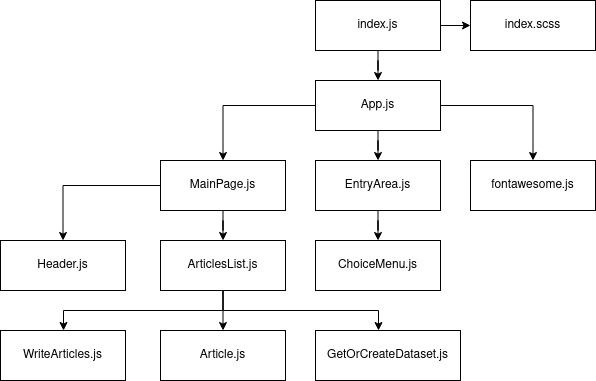
\includegraphics[width=0.87
	\textwidth,  keepaspectratio]{fig/Dependencies}
	\caption{L'albero delle dipendenze dei moduli di {\tt my-solid-blog} contenuti all'interno della directory {\tt src}.}
	\label{fig:bernersLee}
\end{figure}

\bigskip

\section{Gestione delle interfacce grafiche}

\medskip

Importante argomento all'interno di {\tt my-solid-blog} è quello riguardante la renderizzazione delle interfacce grafiche presenti all'interno del progetto. Infatti l'utente deve poter visualizzare differenti interfacce grafiche ad esempio in relazione al fatto che abbia già effettuato l'accesso o meno. 

\bigskip

{\tt React} effettua un rerender dei propri componenti ogni volta che lo stato di un componente cambia. A tale scopo è stato utilizzato l'{\tt hook} {\tt state} di {\tt React}, per poter andare a modificare lo stato dei vari componenti in base alle decisioni prese dall'utente all'interno dell'applicazione.

\bigskip

Innanzitutto va precisato che gli {\tt hooks} sono una feature di {\tt React} aggiunta recentemente; questa permette di utilizzare {\tt state} ed altre features caratteristiche di {\tt React} senza dover necessariamente scrivere una classe, come precedentemente richiesto. Al contrario utilizzando l'{\tt hook} {\tt state}, è stato possibile realizzare l'applicazione {\tt my-solid-blog} senza dover scrivere alcuna classe.

\bigskip

Viene qui di seguito riportato un esempio di codice per l'utilizzo dell'hook {\tt State}.

\medskip

\begin{lstlisting}

import React, { useState } from 'react';
 ... 
const [state, setState] = useState("")
 ... 
\end{lstlisting}

\medskip

La variabile {\tt state}, in questo esempio, rappresenta il valore attuale dello stato, mentre la funzione {\tt setState()} permette di modificare lo stato {\tt state}; il valore contenuto all'interno di {\tt useState()}, in questo esempio {\tt ""}, rappresenta il valore dello stato nel momento in cui tale componente viene caricato per la prima volta.

\bigskip

All'interno del progetto {\tt my-solid-blog}, tale hook è stato, per esempio, utilizzato in {\tt App.js}, per determinare quale interfaccia grafica mostrare all'utente in relazione al fatto che quest'ultimo abbia già completato la procedura di accesso o meno. Viene ora mostrato parte del codice contenuto nel modulo {\tt App.js}.

\medskip

\begin{lstlisting}
import React, { useState } from 'react';
...
function App () {
  const [entered, setEntered] = useState(false);
  const [webId, setWebId] = useState("");
  return (
    <div>
    { !session.info.isLoggedIn && !entered ? (
      <EntryArea
        entering={() => setEntered(true)}
        setWebId={(id) => setWebId(id)}
      />       
    ) : (        
      <MainPage
        webId={webId}
      />
    )}
    </div>
  );
}
\end{lstlisting}

\medskip

Il codice sopra mostrato è un perfetto esempio di come il problema di rerenderizzazione delle interfacce grafiche è stato affrontato all'interno dell'applicazione {\tt my-solid-blog}. In questo caso lo stato {\tt entered} è una variabile booleana pari a {\tt false} nel caso in cui l'utente debba ancora accedere all'applicazione e pari a {\tt true} altrimenti. Lo stato {\tt webId} serve invece per poter salvare la {\tt webId} del proprietario del blog da visualizzare, nel caso in cui non si voglia accedere al proprio blog autenticandosi. Se l'utente non ha ancora effettuato l'accesso all'applicazione, il modulo {\tt App.js} renderizza il componente $<EntryArea>$ che gestisce l'interfaccia grafica dell'applicazione prima di aver effettuato l'accesso, altrimenti viene renderizzato il componente $<MainPage>$ il quale contiene anche l'interfaccia grafica relativa ad ogni singolo articolo. La funzione $() => setEntered(true)$ viene passata al componente $<EntryArea>$ per permettergli di modificare lo stato {\tt entered} di {\tt App.js}. In questo modo {\tt EntryArea.js} può utilizzare tale funzione nel momento in cui l'utente ha effettuato l'accesso al blog appartenente ad una determinata {\tt webId} selezionata. Modificando lo stato {\tt entered}, {\tt EntryArea.js} forza {\tt App.js} a rerenderizzare la propria interfaccia grafica, in modo tale da visualizzare la lista di articoli presenti nel blog selezionato, renderizzando il componente $<MainPage>$.

\bigskip

\section{Container e risorse utilizzati per la gestione del blog}

\medskip

Dalle specifiche dell'applicazione {\tt my-solid-blog} risulta che i dati relativi agli articoli devono essere necessariamente pubblici, in quanto devono essere accessibili anche da parte utenti non autenticati. Infatti, nota la {\tt webId} di un utente, chiunque deve essere in grado di leggere il suo blog tramite l'applicazione {\tt my-solid-blog}.

\bigskip

Da tali considerazioni si evince che il {\tt container} ideale per salvare le informazioni inerenti al blog è il {\tt container} {\tt public}. Tale {\tt container} è normalmente presente di default in ogni {\tt Pod}. Le risorse {\tt ACL} di tale {\tt container} consentono di avere diritto in lettura sulle risorse all'interno di tale {\tt container}; questo significa che le risorse interne a tale {\tt container} possono essere scaricate anche senza essersi precedentemente autenticati con il server {\tt Solid}. Inoltre all'interno del {\tt container} {\tt setting}, anch'esso di norma presente di default all'interno del {\tt Pod}, è contenuto un {\tt SolidDataset} chiamato {\tt publicTypeIndex.ttl} avente lo scopo di tenere traccia di tutti i {\tt SolidDataset} accessibili pubblicamente all'interno del {\tt Pod}; anche la risorsa {\tt publicTypeIndex.ttl} è accessibile pubblicamente in lettura agli utenti non autenticati. L'applicazione {\tt my-solid-blog} salva il proprio {\tt SolidDataset}, chiamato {\tt articlelist.ttl}, all'interno di un {\tt container} chiamato\\ {\tt my-solid-blog}, creato dall'applicazione stessa, e situato a sua volta all'interno del {\tt container} {\tt public} per le considerazioni esposte in precedenza. Poiché {\tt articlelist.ttl} è una risorsa pubblicamente accessibile, {\tt my-solid-blog} riporta all'interno del {\tt SolidDataset} {\tt publicTypeIndex.ttl} alcune informazioni riguardanti {\tt articlelist.ttl}, tra le quali l'URL della risorsa per poterla scaricare tramite {\tt publicTypeIndex.ttl}. Infine l'applicazione legge anche alcuni dati contenuti direttamente all'interno del {\tt SolidDataset} relativo al profilo dell'utente. Il profilo di un utente è anch'esso una risorsa pubblicamente accessibile. Le informazioni lette dal profilo sono, ad esempio, il nome, l'organizzazione di cui fa parte l'utente e il ruolo che ha in tale organizzazione; queste informazioni vengono lette dall'applicazione per poterle mostrare all'utente insieme agli articoli contenuti all'interno del blog.

\bigskip

\section{Scaricamento del SolidDataset articlelist.ttl}

\medskip 

Nel momento in cui l'applicazione viene avviata, essa necessita di scaricare il {\tt SolidDataset} {\tt articlelist.ttl} dal {\tt Pod} dell'utente. I moduli che si occupano di eseguire queste operazioni sono {\tt ArticlesList.js} e {\tt GetOrCreateDataset.js}. Vengono qui di seguito elencate le operazioni eseguite da questi moduli per poter scaricare tale risorsa.

\begin{itemize}
	\item Per prima cosa è necessario conoscere la {\tt webId} dell'utente in questione. La {\tt webId} rappresenta l'URL dell'oggetto chiamato {\tt me} all'interno del profilo dell'utente sul quale vengono memorizzate le informazioni relative all'utente proprietario del {\tt Pod} e alla struttura del {\tt Pod} stesso. Se un utente si è autenticato con il {\tt Solid Identity Provider} allora l'applicazione può leggere la sua {\tt webId} utilizzando l'oggetto {\tt session} e in particolare la proprietà {\tt session.info.webId}. Se l'utente ha effettuato l'accesso senza autenticarsi, allora ha dovuto indicare la {\tt webId} dell'utente proprietario del blog che vuole leggere. Questo significa che, anche in questo caso, l'applicazione conosce la {\tt webId} da utilizzare.
	\item All'interno dell'oggetto {\tt me} è presente l'URL della radice del {\tt Pod}, necessario per poter conoscere l'ubicazione dei {\tt container} {\tt settings} e {\tt public}. Tale informazione è salvata utlizzando il vocabolario {\tt RDF} {\tt http://www.w3.org/ns/pim/space\#}, e in particolare, la proprietà {\tt storage} di tale vocabolario. Come descritto nel precedente capitolo, tale valore può essere letto utilizzando la funzione {\tt getUrl()}.
	\item Il vocabolario {\tt <http://www.w3.org/ns/solid/terms\#>}, ovvero il vocabolario di {\tt Solid}, viene utilizzato all'interno dell'oggetto {\tt me} per salvare l'URL del {\tt SolidDataset}\\ {\tt publicTypeIndex.ttl}; in particolare tale URL viene salvato utilizzando la proprietà {\tt publicTypeIndex} del vocabolario {\tt solid}.
	\item Viene scaricato il {\tt SolidDataset} {\tt publicTypeIndex.ttl}. Tale {\tt SolidDataset}, come in parte già accennato, contiene una lista di oggetti che si riferscono alle risorse accessibili pubblicamente all'interno del {\tt Pod}. L'applicazione usa {\tt publicTypeIndex.ttl} per controllare se esite un oggetto al suo interno che si riferisce ad {\tt articlelist.ttl}.
	\item Se esiste tale oggetto riferito ad {\tt articlelist.ttl}, questo significa che tale {\tt SolidDataset} esiste già all'interno del {\tt Pod}, cioè è stato creato in precedenza. In questo caso l'applicazione deve solamente leggere il valore sotto la proprietà {\tt instance} del vocabolario {\tt solid} per conoscere l'URL sotto il quale {\tt articlelist.ttl} è stato salvato. Una volta noto l'URL di {\tt articlelist.ttl}, l'applicazione può procedere scaricando tale {\tt SolidDataset}.
	\item Nel caso in cui tale oggetto non esista, questo significa che {\tt articlelist.ttl} non è stato inizializzato. L'applicazione deve quindi procedere creando tale risorsa.
	\item Viene quindi composto l'URL della risorsa {\tt articlelist.ttl} da creare, aggiungendo all'URL della radice del {\tt Pod}, precedentemente ottenuto utilizzando l'oggetto {\tt me}, la stringa "public/my-solid-blog/articlelist.ttl".
	\item Il {\tt SolidDataset} in questione viene creato sotto tale URL; tale operazione può essere compiuta solo se l'utente ha effettuato l'accesso all'applicazione completando l'operazione di logging. In caso contrario {\tt my-solid-blog} non possiede il diritto in scrittura necessario per effettuare tale operazione, ed è costretto ad arrestarsi, senza permettere all'utente di visualizzare alcun articolo.
	\item Come ultima operazione viene creato un oggetto all'interno di {\tt publicTypeIndex.ttl}, per poterci salvare l'URL scelto per {\tt articlelist.ttl}. In questo modo l'applicazione potrà utilizzare tale informazione la volta successiva in cui dovrà leggere tale blog per poter scaricare tale {\tt SolidDataset}.
\end{itemize}

\bigskip

\section{Struttura di articlelist.ttl}

\medskip

{\tt articlelist.ttl} contiene al suo interno vari oggetti, ognuno dei quali si riferisce ad un articolo differente pubblicato all'interno del {\tt Pod}. Nel momento in cui si accede all'interno di {\tt my-solid-blog}, l'applicazione permette all'utente di visualizzare la lista di articoli presenti all'interno di tale {\tt SolidDataset}. 

\medskip

I singoli articoli sono stati definiti utilizzando il vocabolario {\tt RDF} {\tt http://schema.org/}, in particolare sono state utilizzate le seguenti proprietà e classi di tale vocabolario.

\begin{itemize}
	\item Ogni oggetto-articolo è un'istanza della classe {\tt TextDigitalDocument}, classe definita, appunto, nel vocabolario {\tt schema}; tale classe ha lo scopo di rappresentare file composti prevalentemente da testo.
	\item La proprietà {\tt dataCreated}, viene utizzata per indicare la data di creazione dell'articolo.
	\item La proprietà {\tt headline} indica il titolo dell'articolo.
	\item La proprietà {\tt text} è utilizzato per poter salvare il contenuto di un articolo.
	\item Infine la proprietà {\tt identifier} viene utilizzata per poter identificare univocamente ogni articolo presente in {\tt articlelist.ttl}.
\end{itemize}

\medskip

Come indicato all'interno della lista delle specifiche, l'applicazione mostra all'utente il titolo, la data e il contenuto di ogni articolo. L'identifier viene invece utilizzato come chiave di {\tt React}, per poter permettere a {\tt React} di renderizzare correttamente la lista di articoli presenti. Infine, su richiesta dell'utente, {\tt my-solid-blog} visualizza all'utente l'URL in cui la risorsa relativa al singolo articolo è stata memorizzata. Tale funzione, come verrà spiegato in seguito, è necessaria per permettere all'utente di interagire correttamente con il server {\tt blog-validator}.
\bigskip

\section{Gestione degli articoli}

\medskip

Come già in parte accennato, i moduli che si occuppano di gestire e renderizzare la lista di articoli presenti all'interno del blog sono: {\tt ArticlesList.js} e {\tt Article.js}.

\bigskip

Nel dettaglio {\tt Articleslist.js} si occupa di scaricare il {\tt SolidDataset}\\{\tt Articlelist.ttl}, di renderizzare e gestire la lista di articoli presenti importando {\tt Article.js}, di aggiungere nuovi articoli alla lista per gli utenti autenticati, di definire le funzioni per poter modificare o eliminare un articolo e di passare alcune informazioni come parametri necessari alla gestione dei singoli articoli ad {\tt Article.js}.

\bigskip

Il modulo {\tt Article.js} invece ha i seguenti compiti: renderizzare i singoli articoli contenuti all'interno del blog, utilizzare le funzioni definite in {\tt ArticlesList.js} per permettere agli utenti autenticati di modificare o cancellare un articolo, consentire a {\tt my-solid-blog} e {\tt blog-validator} di comunicare tra di loro per verificare l'autenticità dei singoli articoli mostrati da {\tt my-solid-blog}.

\bigskip

Una volta caricato il {\tt SolidDataset} {\tt Articlelist.ttl}, il modulo {\tt ArticlesList.js} utilizza la funzione {\tt getThingAll()} della libreria {\tt solid-client} per poter ottenere un array contenente tutti gli articoli del blog. Tale array viene quindi ordinato in base alla data di creazione degli articoli stessi, utilizzando la funzione {\tt byDate()}, anch'essa definita all'interno di {\tt ArticlesList.js}. Una volta che tale operazione è terminata, viene eseguito il metodo {\tt map()} sull'array precedentemente ottenuto, in modo tale da renderizzare il contenuto dei singoli articoli utilizzando il modulo {\tt Article.js}; tale funzione {\tt map()} ritorna il singolo componente $<Article>$ per ogni elemento presente all'interno dell'array. Al componente $<Article>$ vengono passati i seguenti argomenti:

\begin{itemize}
	\item {\tt thing}: oggetto rappresentante il singolo articolo all'interno del blog; tramite esso è possibile leggere e modificare le informazioni relative al singolo articolo.
	\item {\tt remove}: funzione che permette all'utente autenticato di eliminare un articolo all'interno del blog. Questa funzione asincrona riceve in ingresso l'oggetto, ovvero l'articolo, da eliminare da {\tt articlelist.ttl}; una volta eliminato la funzione salva all'interno del {\tt Pod} il {\tt SolidDataset} aggiornato.
	\item {\tt change}: funzione asincrona avente lo scopo di modificare il contenuto di un articolo: in particolare permette all'utente autenticato di modificare titolo e contenuto dell'articolo. Riceve in ingresso l'oggetto da modificare, il nuovo titolo e il nuovo contenuto. Una volta che l'articolo viene aggiornato la funzione salva all'interno del {\tt Pod} il {\tt SolidDataset} aggiornato.
	\item {\tt webId}: variabile contenente la {\tt webId} del proprietario del blog. Tale variabile viene utilizzata solamente se l'utente ha effettuato l'accesso senza autenticarsi; in caso contrario la {\tt webId} può essere letta direttamente da {\tt session.info.webId}.
\end{itemize}

\bigskip

{\tt Article.js} mette quindi a disposizione due componenti $<button>$ per permettere all'utente di modificare ed eliminare l'articolo renderizzato; tali componenti vengono visualizzati dall'utente solo se la variabile {\tt session.info.isLoggedIn} è pari a {\tt true}, cioè solamente se l'utente si è correttamente autenticato con il proprio {\tt Solid Identity Provider}.

\bigskip


\section{Comunicazione con l'applicazione blog-validator}

\medskip

Per effettuare un controllo sull'autenticità dei contenuti mostrati all'interno del blog dell'utente, l'applicazione {\tt my-solid-blog} comunica attraverso il protocolo {\tt HTTP} con il server {\tt blog-validator}.

\bigskip

A tale proposito viene utilizzato il metodo {\tt POST} per effettuare una richiesta a\\{\tt blog-validator}, dopodichè {\tt my-solid-blog} aspetta la risposta del server per poter mostrare all'utente l'esito di tale controllo.

\bigskip


Per inviare tale richiesta {\tt POST} al server, come già esposto all'interno del capitolo 2, l'applicazione {\tt my-solid-blog} fa uso della libreria {\tt axios}; in particolare utilizza il metodo {\tt axios.post()}; tale metodo ritorna all'applicazione una promessa. L'applicazione\\{\tt my-solid-blog} rimane in attesa che tale promessa si risolva o venga rifiutata. Nel caso in cui si risolva, allora questo significa che la comunicazione con il server è andata a buon fine. In questo caso l'applicazione può quindi mostrare all'utente l'esito del controllo effettuto da {\tt blog-validator}; in caso contrario, qualora la promessa venga rifiutata, si è verificato un errore durante tale comunicazione.

\bigskip

Per poter comunicare l'applicazione {\tt my-solid-blog} utilizza la porta {\tt 3000}, mentre {\tt blog-validator} utilizza la porta {\tt 8081}. Gli argomenti passati alla funzione {\tt axios.post()} sono i seguenti: l'URL su cui il server è in ascolto, che è pari a {\tt http://localhost:8081/auth} e tutte le informazioni necessarie al server per effettuare tale controllo attraverso un file formato {\tt JSON}. In particolare le proprietà presenti all'interno di tale file JSON sono le seguenti:

\begin{itemize}
	\item {\tt webId}: viene passata a {\tt blog-validator} la {\tt webId} del proprietario del {\tt Pod}. La {\tt webId} del proprietario è necessaria a comprendere se il server ha cercato le informazioni all'interno del {\tt Pod} corretto.
	\item {\tt urlDataset}: URL relativo al {\tt SolidDataset} da scaricare; {\tt my-solid-blog} invia, infatti, a {\tt blog-validator} l'URL relativo a {\tt articlelist.ttl}, per poterlo scaricare e poter leggere i dati al suo interno.
	\item {\tt urlThing}: URL in cui la risorsa relativa all'articolo è stata memorizzata, permette al server di trovare l'articolo in questione all'interno del {\tt SolidDataset}, nel caso in cui questo esista effettivamente all'interno di {\tt articlelist.ttl}.
	\item {\tt title}: titolo dell'articolo, necessario per controllare che questo non sia stato alterato da {\tt my-solid-blog}.
	\item {\tt content}: contenuto dell'articolo, inviato per le stesse motivazioni della proprietà {\tt title}.
	\item {\tt date}: data di creazione dell'articolo; è necessario inviare tale informazione per controllare che anche questo dato non sia stato manomesso in nessun modo dall'applicazione.
\end{itemize}

\bigskip

L'applicazione invia tale richiesta {\tt POST} a {\tt blog-validator} ogni volta che si preme il pulsante chiamato {\tt Check}, situato al di sotto di ogni articolo renderizzato da {\tt my-solid-blog}. L'esito del controllo viene anch'esso stampato al di sotto dell'articolo controllato.


\bigskip

\section{Utilizzo dell'hook Effect}

\bigskip

Oltre all'{\tt hook} {\tt State}, l'aplicazione {\tt my-solid-blog} utilizza un altro {\tt hook} di {\tt React}, chiamato {\tt Effect}, anch'esso aggiunto recentemente. Tale {\tt hook} è utilizzato per implementare side effects all'interno dei componenti delle funzioni. Esempi di side effects  all'interno dei componenti {\tt React} sono: il download di dati, l'impostazione di una iscrizione o il cambiamento manuale del {\tt DOM}.

\bigskip

Talvolta, quando si utilizza {\tt React} è necessario eseguire del codice aggiuntivo, dopo che {\tt React} ha aggiornato il {\tt DOM}. {\tt useEffect} serve ad informare i vari componenti {\tt React}, su cosa questi sono tenuti a fare una volta terminata l'operazione di renderizzazione delle interfacce grafiche. {\tt React} memorizza la funzione passata a questo {\tt hook} e la esegue in un secondo momento, ovvero dopo che il {\tt DOM} è stato aggiornato. Il codice all'interno {\tt useEffect} viene di default eseguito ogni volta che {\tt React} termina l'operazione di render. Questo hook è utilizzato all'interno di {\tt my-solid-blog} per scaricare il {\tt SolidDataset} {\tt articlelist.ttl}; infatti scaricare dati dalla rete è un tipico side effect da eseguire tramite {\tt Effect}. Per chi ha familiarità con le classi {\tt React}, l'{\tt hook} {\tt useEffect} sostituisce i metodi {\tt componentDidMount}, {\tt componentDidUpdate } e {\tt componentWillUnmount} delle classi {\tt React}.

\bigskip

Nel caso di {\tt my-solid-blog}, viene passata all'{\tt hook} {\tt useEffect} non solo la funzione da eseguire, ma anche l'array {\tt [session]}. Questo permette di ottimizzare l'applicazione, in quanto, passando questo argomento, la funzione all'interno di {\tt useEffect} non viene più eseguita al termine di ogni renderizzazione da parte di {\tt React}, ma soltanto quando uno o più elementi dell'array {\tt [session]}, fra un render e l'altro, sono cambiati.

\bigskip

\section{Link a blog-validator}

\medskip

All'interno dell'applicazione, come già precedentemente detto, è possibile inviare, tramite procollo {\tt HTTP}, una richiesta {\tt POST} al server {\tt blog-validator}, con il fine di evitare la diffusione di informazioni false all'interno dell'applicazione {\tt my-solid-blog}. Per effettuare tale controllo {\tt my-solid-blog} invia a {\tt blog-validator} alcune informazioni riguardanti i dati relativi all'articolo in questione. Una volta terminata la comunicazione con il server, l'applicazione {\tt my-solid-blog}, infine mostra all'utente l'esito del controllo effettuato da {\tt blog-validator}. Tuttavia l'utente, non avendo modo di vedere in prima persona i dati scambiati tra le due applicazioni, non può avere certezze riguardo i seguenti aspetti:

\begin{itemize}
	\item L'utente non può verificare se l'applicazione {\tt my-solid-blog} abbia effettivamente inviato correttamente i dati relativi all'articolo in questione. {\tt my-solid-blog} potrebbe inviare intenzionalmente dati relativi ad un altro articolo, per poter andare a modificare l'esito del controllo effettuato da {\tt blog-validator}.
	\item L'applicazione {\tt my-solid-blog} potrebbe far credere all'utente che {\tt blog-validator} non abbia rilevato anomalie durante il controllo, visualizzando a questo un esito differente da quello effettivamente rilevato dal server.
\end{itemize}

\medskip

Per evitare tale problema all'interno dell'applicazione {\tt my-solid-blog} è possibile trovare un link per potersi connettere direttamente con {\tt blog-validator} tramite browser. Visitando tale URL, l'utente può vedere quali sono stati realmente i dati inviati da {\tt my-solid-blog} a {\tt blog-validator} insieme al reale esito di tale controllo. In questo modo l'utente può verificare in prima persona se il controllo sull'autenticità degli articoli mostrati da {\tt my-solid-blog} può ritenersi valido o meno.

\clearpage

\textbf{Vengono ora descritte le modalità di funzionamento e l'implementazione dell'applicazione blog-validator.}

\bigskip

{\tt blog-validator} è un server implementato tramite {\tt Node.js}, utilizzato per controllare l'autenticità dei dati mostrati dall'applicazione {\tt my-solid-blog}; {\tt blog-validator} utilizza la porta 8081.

\bigskip


\section{Directory e file presenti in blog-validator}

\medskip

Sono qui di seguito elencati tutti i file e le directory presenti all'interno del progetto {\tt blog-validator}.

\medskip

La cartella {\tt node-modules} e i file {\tt package-lock.json} e {\tt package.json}, presenti all'interno dell'applicazione {\tt blog-validator}, sono già stati trattati in quanto presenti anche all'interno del progetto {\tt my-solid-blog}; per questo motivo non verranno ripetute le loro funzioni all'interno di questa sezione.

\begin{itemize}
	\item {\tt index.js}: file entry point {\tt JavaScript} del progetto {\tt blog-validator}. Definisce alcuni URL per effettuare richieste {\tt GET} e {\tt POST} da parte di terze applicazioni.
	\item {\tt solid.db}: Database utilizzato da {\tt blog-validator} per salvare alcuni dati 
	necessari per il funzionamento dell'applicazione.
	\item {\tt utils}: Directory contenente i moduli {\tt solidRequest.js} e {\tt requestsData.js}.
	\item {\tt solidRequest.js}: File utilizzato per leggere alcuni dati all'interno del {\tt Pod} dell'utente. La lettura di tale dati è necessaria per poter effettuare controlli riguardanti l'autenticità dei dati visualizzati da {\tt my-solid-blog}.
	\item {\tt requestsData.js}: Modulo per la gestione del database {\tt solid.db}, si occupa della creazione di tabelle, dell'inserimento di tuple, e della lettura di alcuni dati all'interno di tale database.
\end{itemize}

\medskip

\bigskip

\section{Tecnologie utilizzate per il funzionamento di blog-validator}

\medskip

Vengono ora brevemente descritti alcuni moduli fondamentali per il funzionamento del server {\tt blog-validator}.

\clearpage

\textbf{Express}

\bigskip

{\tt Express} è un framework per applicazioni web Node.js che fornisce una serie di funzioni avanzate per le applicazioni web e per dispositivi mobili; è ormai definito come il server framework standard de facto per {\tt Node.js}. Tale framework permette la creazione di {\tt API} in maniera semplice e veloce.

\bigskip

\textbf{cookie-session}

\bigskip

I {\tt Session cookies} sono i cookie temporanei che vengono generati principalmente sul lato server, il cui uso principale è quello di tenere traccia di tutte le informazioni della richiesta che è stata fatta dal cliente in una particolare sessione. La sessione viene memorizzata solo temporaneamente, quando l'utente chiude la sessione del browser costui la distrugge in automatico. 

\medskip

Il modulo {\tt express-session} chiamato {\tt cookie-session} è usato per la gestione delle sessioni in {\tt Node.js}.

\bigskip

\textbf{body-parser}

\bigskip

{\tt body-parser} è una libreria {\tt npm} usata per processare i dati inviati al server attraverso un metodo di richiesta {\tt HTTP}.

\bigskip

\textbf{sqlite3}

\bigskip

Libreria {\tt npm} utilizzata per la creazione e la gestione del database utilizzato da {\tt blog-validator}.

\bigskip

\section{API methods di blog-validator}

\medskip

Vengono ora elencati gli API methods messi a disposizione da {\tt blog-validator}.

\begin{itemize}
	\item {\tt POST}, {\tt http://localhost:8081/auth}: Questo metodo è utilizzato dall'applicazione {\tt my-solid-blog} per inviare al server i dati necessari a controllare i dati richiesti dall'utente. I dati ricevuti da {\tt my-solid-blog} vengono poi passati al modulo {\tt solidRequest.js}, il quale si occupa di confrontare le informazioni ricevute con quelle presenti all'interno del {\tt Pod}. I dati inviati da {\tt my-solid-blog} vengono salvati nel database {\tt solid.db}.
	\item {\tt GET}, {\tt http://localhost:8081/check}: Tale metodo è utilizzato per permettere all'utente di interagire con l'applicazione. Consente all'utente di controllare un articolo, una volta noti gli URL del suo {\tt SolidDataset} e dell'articolo stesso, o di controllare il corretto svolgimento di un controllo sull'autenticità dei dati effettuato da {\tt blog-validator} attraverso l'API method {\tt POST}, {\tt http://localhost:8081/auth}, con il fine di verificare che {\tt my-solid-blog} non abbia inviato al server dati scorretti.
	\item {\tt POST}, {\tt http:localhost:8081/control}: Metodo utilizzato per inviare all'utente i dati relativi al controllo sul quale è stata richiesta una verifica. Attraverso il modulo {\tt requestsData.js}, utilizza il database {\tt solid.db} per caricare tali dati richiesti.
	\item {\tt POST}, {\tt http:localhost:8081/read}:  Metodo utilizzato per inviare all'utente i dati relativi ad un articolo, ovvero titolo, contenuto e data di pubblicazione, salvato all'interno del {\tt Pod}. Tale metodo può essere utilizzato per verificare che tali dati coincidano con quelli visualizzati da {\tt my-solid-blog}.
\end{itemize}

\bigskip

\section{Controllo sull'autenticità dei dati}

\medskip

Viene ora descritto nel dettaglio il procedimento, effettuato da {\tt blog-validator}, per controllare l'autenticità dei dati riguardanti un articolo mostrato dall'applicazione {\tt my-solid-blog}. L'articolo sul quale effettuare il controllo viene scelto direttamente dall'utente che sta utilizzando {\tt my-solid-blog}.

\begin{itemize}
	\item Come già indicato precedentemente, quando un utente che sta utilizzando l'applicazione {\tt my-solid-blog} preme il pulsante "Check", {\tt my-solid-blog} invia una richiesta {\tt POST} utilizzando il metodo {\tt http://localhost:8081/auth}. {\tt blog-validator} riceve quindi tutti i dati necessari per verificare l'autenticità dell'articolo, selezionato dall'utente, mostrato da {\tt my-solid-blog}.
	\item I dati ricevuti vengono passati alla funzione {\tt readSolidData()} esportata dal modulo {\tt solidRequest.js}.
	\item Poiché l'applicazione {\tt my-solid-blog} ha passato al server la proprietà {\tt urlDataset}, il quale indica l'URL ove è situato il {\tt SolidDataset} contente l'articolo da controllare, {\tt readSolidData()} può scaricare tale {\tt SolidDataset} utilizzando le funzioni messe a disposizione dalla libreria di {\tt Inrupt} {\tt solid-client}. 
	\item Una volta scaricato il {\tt SolidDataset} in questione, attraverso la proprietà {\tt urlThing}, anch'essa ricevuta da {\tt my-solid-blog}, la quale rappresenta l'URL corrispondente all'articolo in questione, {\tt readSolidData()} può andare a cercare l'oggetto all'interno del {\tt SolidDataset} scaricato che si riferisce a tale articolo.
	\item Se l'articolo in questione non esiste {\tt blog-validator} restituisce a {\tt my-solid-blog}:
	
	\smallskip
	
	{\tt "Article not found: " + req.body.webId + " is not the author"}
	\item Se, invece, l'articolo esiste all'interno del {\tt Pod}, {\tt readSolidData()} legge il titolo e il contenuto di tale articolo e li confronta con quelli che ha ricevuto da {\tt my-solid-blog}.
	\item Se il titolo e/o il contenuto dell'articolo non corrispondono a quelli inviati da {\tt my-solid-blog}, {\tt blog-validator} restituisce a {\tt my-solid-blog} la seguente risposta:
	
	\smallskip
	
	{\tt "Article of " + req.body.webId + " found, but the title or the content are different"}
	\item Se il titolo e il contenuto dell'articolo corrispondono a quelli ricevuti da {\tt my-solid-blog}, {\tt readSolidData()} confronta la data di pubblicazione dell'articolo con quella ricevuta da {\tt my-solid-blog}.
	\item Se queste non corrispondono, {\tt blog-validator} invia a {\tt my-solid-bog} la risposta:
	
	\smallskip
	
	{\tt "Article of " + req.body.webId + " found, but the date is different, the real date is: " + date}
	\item Se c'è corrispondenza anche sulla data di pubblicazione dell'articolo allora {\tt blog-validator} invia a {\tt my-solid-blog} come risposta:
	
	\smallskip
	
	{\tt "Article of " + req.body.webId + " found, all in order"}
	
	\smallskip
	
	Arrivati a questo punto {\tt blog-validator} ha quindi terminato di controllare l'autenticità dell'articolo in questione.	
\end{itemize}

\medskip

Il corretto funzionamento della procedura sopra descritta è stata testata tramite il programma {\tt Postman}.

\bigskip

\section{Gestione del database solid.bd}

\medskip

{\tt blog-validator}, a seguito delle operazioni sopra descritte, utilizza la libreria {\tt sqlite3}, per salvare all'interno del database {\tt solid.db} i dati relativi alle richieste che sono state effettuate da {\tt my-solid-blog}. Tale database è molto semplice e presenta un'unica tabella chiamata {\tt userAuth}; all'interno di questa vengono salvate le informazione necessarie per permettere all'utente di verificare in prima persona che la comunicazione tra {\tt blog-validator} e {\tt my-solid-blog} sia avvenuta correttamente, senza che i dati relativi a tale comunicazione siano stati volontariamente manipolati da quest'ultima applicazione.

\bigskip

Ogni tupla della tabella {\tt userAuth} rappresenta un singolo controllo richiesto dall'applicazione {\tt my-solid-blog} attraverso il metodo {\tt POST} : {\tt http://localhost:8081/auth}. All'interno della tabella {\tt userAuth} sono presenti i seguenti attributi:

\begin{itemize}
	\item {\tt webId}: la {\tt webId} del proprietario del blog.
	\item {\tt urlDataset}: URL del {\tt SolidDataset} dove è memorizzato il blog. Tale {\tt SolidDataset} corrisponde con il Dataset {\tt articlelist.ttl} precedentemente trattato.
	\item {\tt urlThing}: URL corrispondente all'articolo sul quale è stato richiesto il controllo.
	\item {\tt title}: titolo dell'articolo.
	\item {\tt content}: contenuto dell'articolo.
	\item {\tt date}: data di pubblicazione dell'articolo.
	\item {\tt checkDate}: data nella quale è stato richiesto il controllo dall'utente.
	\item {\tt result}: esito del controllo.
\end{itemize}

Tutti i seguenti attributi elencati sono di tipo {\tt TEXT}.

\bigskip 

\section{Il metodo GET, http://localhost:8081/check}

\medskip

Utilizzando l'API method {\tt GET, http://localhost:8081/check} l'utente ha modo di visualizzare i dati contenuti in tale database. Tale link, come già precedentemente indicato, è presente anche all'interno dell'applicazione {\tt my-solid-blog}. Visitandolo un utente può inserire l'URL relativo ad un articolo per poter visualizzare i dati, salvati all'interno del database, relativi al controllo più recente che è stato richiesto su tale articolo. In alternativa, come già indicato, l'utente può digitare l'URL di un articolo e del {\tt SolidDatatset} in cui è salvato, per controllare manualmente il contenuto di tale articolo.

\bigskip

Il motivo per cui {\tt my-solid-blog} mette a disposizione dell'utente il link\\{\tt http://localhost:8081/check} è quello di provare a quest'ultimo che l'applicazione sta rispettando i criteri relativi alla tecnologia {\tt Solid}: l'applicazione, infatti, non salva localmente nessun dato relativo all'utente, ma utilizza unicamente i dati contenuti all'interno del {\tt Pod} dell'utente proprietario del blog.

\bigskip

\section{Possibili futuri miglioramenti del sistema SADeB}

\medskip

In questa sezione sono elencate alcune ulteriori funzionalità del sistema {\tt SADeB} che, per alcune motivazioni, non sono state implementate.

\begin{itemize}
	\item Quando si effettua un controllo su un articolo, {\tt my-solid-blog} potrebbe inviare a {\tt blog-validator} soltanto l'hash relativo al titolo e al contenuto di un articolo. Utilizzando, per esempio, l'algoritmo {\tt SHA-256}, il quale permette di generare {\tt digest} di lunghezza 256 bit per comunicare con il server {\tt blog-validator}, la comunicazione attraverso il protocollo {\tt HTTP} risulterebbe essere più veloce. In questo caso al server basterebbe soltanto confrontare l'hash inviatogli da {\tt my-solid-blog} con quello del titolo o del contenuto dell'articolo, per stabilire l'autenticità o meno dei contenuti postati all'interno del blog.
	\item Poiché {\tt Solid} permette ai propri utenti di memorizzare anche file all'interno del proprio {\tt Pod}, l'applicazione {\tt my-solid-blog} potrebbe in futuro permettere agli utenti di caricare un'immagine per il proprio blog, salvandola nel {\tt Pod}, e di consentire di visualizzarla ogni volta che un qualsiasi altro utente visiti il profilo. Attualmente {\tt Inrupt} mette a disposizione alcune funzioni all'interno della libreria {\tt solid-client} per poter leggere e scrivere file contenuti nel proprio {\tt Pod}.
	\item L'applicazione {\tt blog-validator} potrebbe memorizzare i dati relativi ai controlli richiesti dal client tramite la tecnologia {\tt Solid}, anziché utilizzare un {\tt database} locale. In questo caso sarebbe necessario trovare uno o più vocabolari {\tt RDF} per poter rappresentare tale tipologia di dati. Nel caso in cui non esistessero vocabolari adatti a tale scopo, sarebbe necessario scriverne uno e pubblicarlo all'interno del {\tt container} {\tt public} presente all'interno del {\tt Pod}. In questo modo il vocabolario risulterebbe accessibile ed utilizzabile anche da altri utenti che hanno la necessità di rappresentare la stessa tipologia di dati descritta all'interno di tale ipotetico vocabolario.
	\item L'applicazione {\tt my-solid-blog} potrebbe permettere di creare blog appartenenti a gruppi di utenti, anziché ad uno singolo; in questo caso il blog sarebbe formato dai vari articoli appartenenti agli utenti. Attraverso il vocabolario {\tt ACL}, che {\tt Solid} utilizza per determinare i livelli di permesso concessi ad un utente o ad un'applicazione all'interno di un {\tt Pod}, ogni utente potrebbe decidere quali altre persone oltre a lui possano modificare gli articoli presenti nel proprio {\tt SolidDataset} riferito al {\tt Pod}. Attualmente la documentazione relativa alla gestione delle {\tt Access Control List} in {\tt Solid} è limitata e soggetta a frequenti cambiamenti.
\end{itemize}	


\clearpage


\chapter{Conclusioni e sviluppi futuri}

\medskip

{\tt Solid} è una tecnologia che nasce a seguito della presa visione di un grave problema riguardante il web, ovvero quello relativo alla perdita di privacy da parte degli utenti di internet. La tecnologia {\tt Solid} mira a risolvere tale problema in maniera molto innovativa, attraverso un nuovo modo di concepire lo stesso web. I vantaggi, da parte dell'utente, nell'utilizzo di applicazioni decentralizzate risultano essere molteplici: in primo luogo attraverso l'utilizzo di {\tt Solid}, viene superato il problema relativo alla perdita di privacy e al controllo dei dati dell'utente da parte delle grandi multinazionali di internet. Inoltre, rappresentando i dati contenuti all'interno dei {\tt Pod} attraverso un unico linguaggio, ovvero {\tt RDF}, è possibile permettere a qualsiasi tipo di applicazione di collaborare nella creazione di un'unica struttura di dati condivisa, in quanto tutti i dati relativi alle applicazioni decentralizzate vengono salvati utilizzando il medesimo formato. La separazione del piano delle applicazioni da quello dei dati, auspicata da Berners-Lee, comporterebbe inoltre per l'utente la possibilità di poter scegliere quali applicazioni web utilizzare, basandosi unicamente sulla qualità del servizio offerto dall'applicazione stessa; infatti, non avendo quest'ultima il controllo dei dati relativi all'utente, non può in alcun modo reclamare i dati che sono già stati salvati all'interno del {\tt Pod}. Da queste considerazioni si può concludere che è possibile, se non auspicabile, che in futuro {\tt Solid}, o un'altra tecnologia simile a questa, possa diventare di uso comune, rimpiazzando l'attuale modello utilizzato per l'interazione con le applicazioni web, il quale prevede la consegna dei propri dati personali in cambio dell'utilizzo gratuito del servizio offerto.

\bigskip

L'apprendimento della programmazione di applicazioni decentralizzate in accordo con questa tecnologia, non è stato per me banale: per poter imparare a programmare applicazioni {\tt Solid} è stato infatti necessario, prima di tutto, imprare a conoscere alcuni linguaggi di programmazione come {\tt HTML}, {\tt CSS} e {\tt JavaScript}, fondamentali per lo sviluppo di applicazioni web, e le tecnologie {\tt React} e {\tt Node.js}. In secondo luogo è stato, ovviamente, necessario imparare a padroneggiare il linguaggio {\tt RDF}, e ad utilizzare le librerie messe a disposizione da {\tt Inrupt}. Oltre a queste considerazioni, è bene anche precisare che, essendo una tecnologia in via di sviluppo, non è presente ancora una documentazione particolarmente dettagliata che consenta di imparare agevolmente a programmare applicazioni decentralizzate tramite {\tt Solid}. Inoltre attualmente non esiste ancora una grande comunità di sviluppatori dietro ad essa; pertanto spesso risulta difficile trovare un supporto in caso di difficoltà. È bene anche menzionare il fatto che, essendo una tecnologia in pieno sviluppo, alcuni aspetti chiave relativi ad essa, come il {\tt Solid Protocol} o il {\tt Web Access Control} citati nei capitoli precedenti, sono ancora soggetti a frequenti modifiche, non avendo attualmente raggiunto uno stadio definitivo. Ovviamente questo comporta allo stato attuale alcune difficoltà allo sviluppatore nel programmare applicazioni in accordo con questa tecnologia. A titolo di esempio all'interno dell'applicazione {\tt my-solid-blog} non è stato per me possibile andare a creare e modificare le risorse {\tt ACL} relative al blog per stabilire livelli di permesso intermedi ad altri utenti; questa funzionalità non è stata, infatti, implementata a causa dello scarso materiale messo a disposizione dagli sviluppatori per imparare a gestire questa particolare tipologia di risorse. Attualmente infatti non esiste una guida sufficientemente dettagliata per risolvere tale problema; per esempio, all'interno della documentazione relativa alla libreria {\tt solid-client} di {\tt Inrupt}, è possibile leggere le seguenti frasi nella descrizione di ogni funzione finalizzata alla gestione delle risorse {\tt ACL}: "La specifica Web Access Control non è ancora stata finalizzata. Come tale, questa funzione è ancora sperimentale e soggetta a cambiamenti, anche in una non-major release" \cite{inruptdoc}. Le problematiche sopra enunciate riguardo alla gestione delle risorse {\tt ACL} hanno fatto sì che l'applicazione {\tt my-solid-blog} abbia potuto usufruire soltanto delle risorse {\tt ACL} di default, contenute all'interno del {\tt Pod}, non potendo andarne a creare delle nuove.

\bigskip

Nonostante le problematiche sopra elencate, {\tt Solid} rimane una tecnologia dal potenziale enorme, in grado di risolvere uno dei problemi più importanti della società di oggi, ovvero quello relativo alla perdita di privacy e alla diffusione di disinformazione online. {\tt Solid} ha acquisito, a partire dalla sua nascita, uno sviluppo e una popolarità sempre maggiori e probabilmente questo andamento continuerà a proseguire nei prossimi anni. In considerazione di quanto esposto all'interno di questo capitolo e di quelli precedenti, mi sento di poter affermare che  una tecnologia come {\tt Solid} è di vitale importanza per migliorare una delle più grandi invenzioni del secolo: il {\tt World Wide Web}, e che nell'utilizzare tale tecnologia gli utenti internet possono trarne grandi benefici.



\clearpage
%...

%%APPENDICI==============================================
\appendix
%%\input{appendiceA}
%...

%%BIBLIOGRAFIA============================================
\normalsize
\newpage
\bibliographystyle{plain}
\bibliography{bibliografia}

\end{document}
